\subsection*{一、光學量測器材}
\begin{table}[H]
    \setlength{\extrarowheight}{1pt}
    \centering

    \begin{tabular}{|m{2cm}|m{3cm}|m{3cm}|m{3cm}|}
        \hline
        \centering 名稱 & \centering 氦氖雷射 & \centering TSL2591 感光元件 & \centering Arduino Uno  \tabularnewline \hline
        \centering 圖片 & 
        \centering 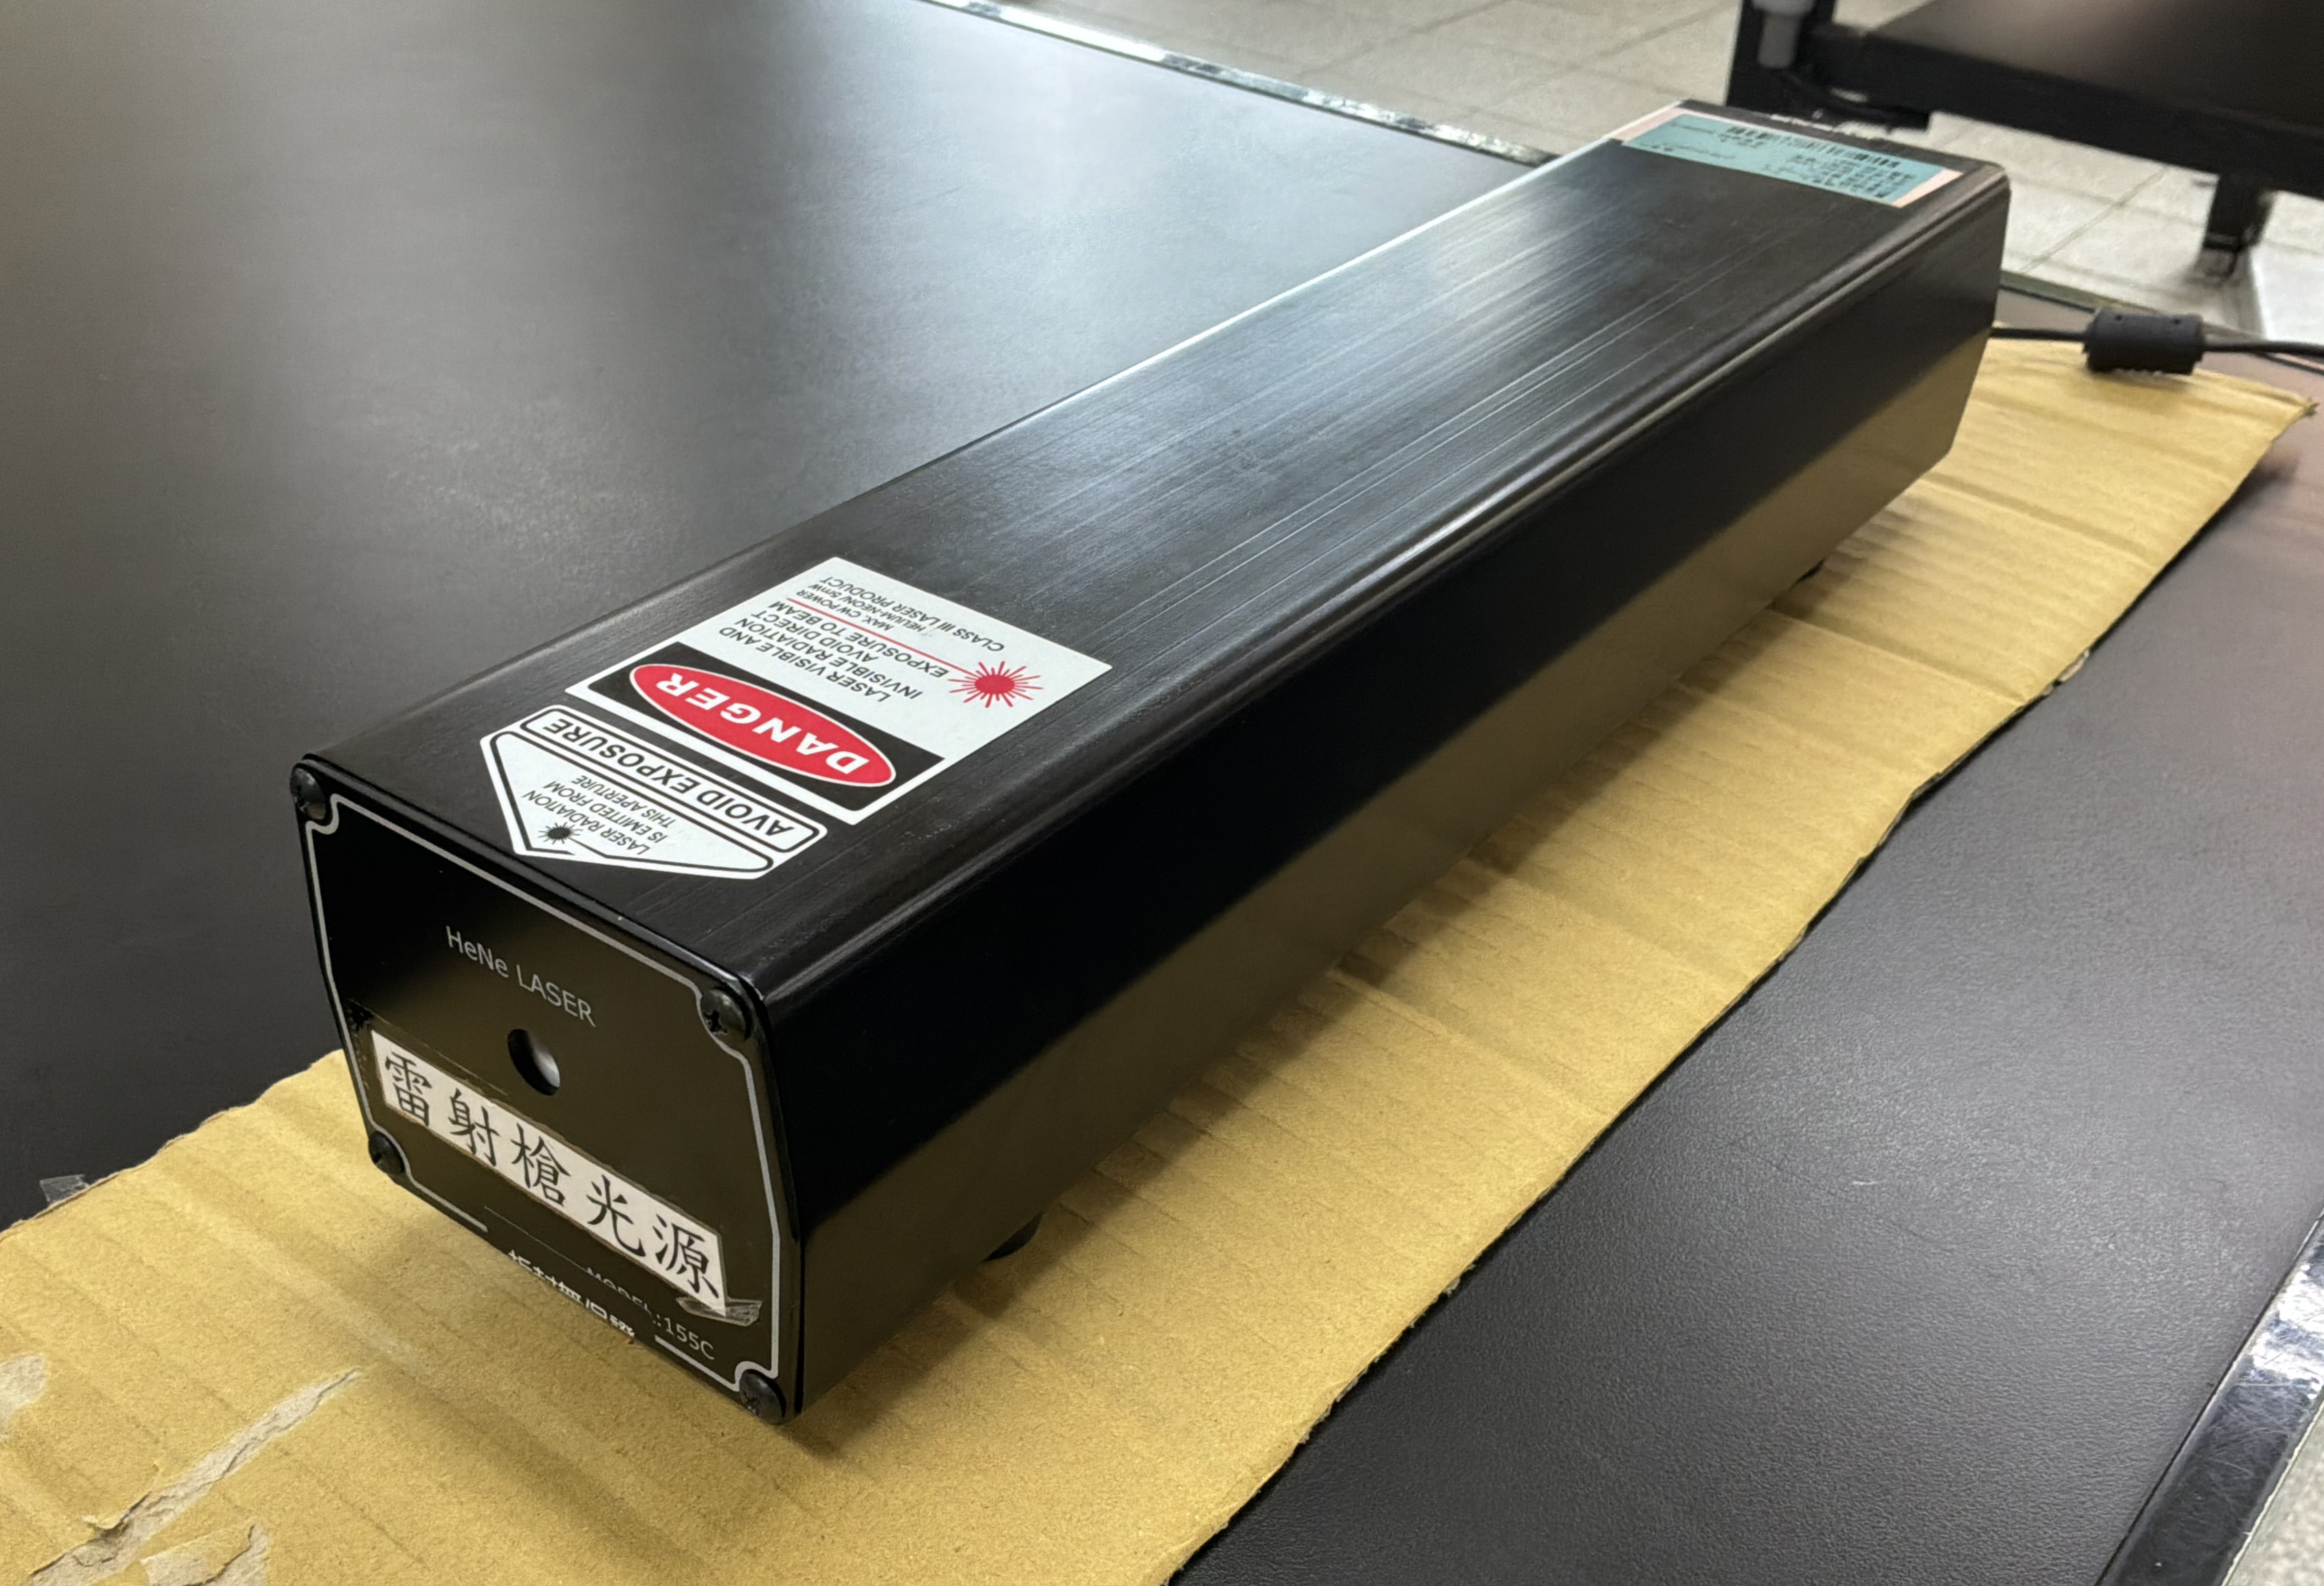
\includegraphics[width=3cm, align=c]{image/雷射槍.png} & 
        \centering 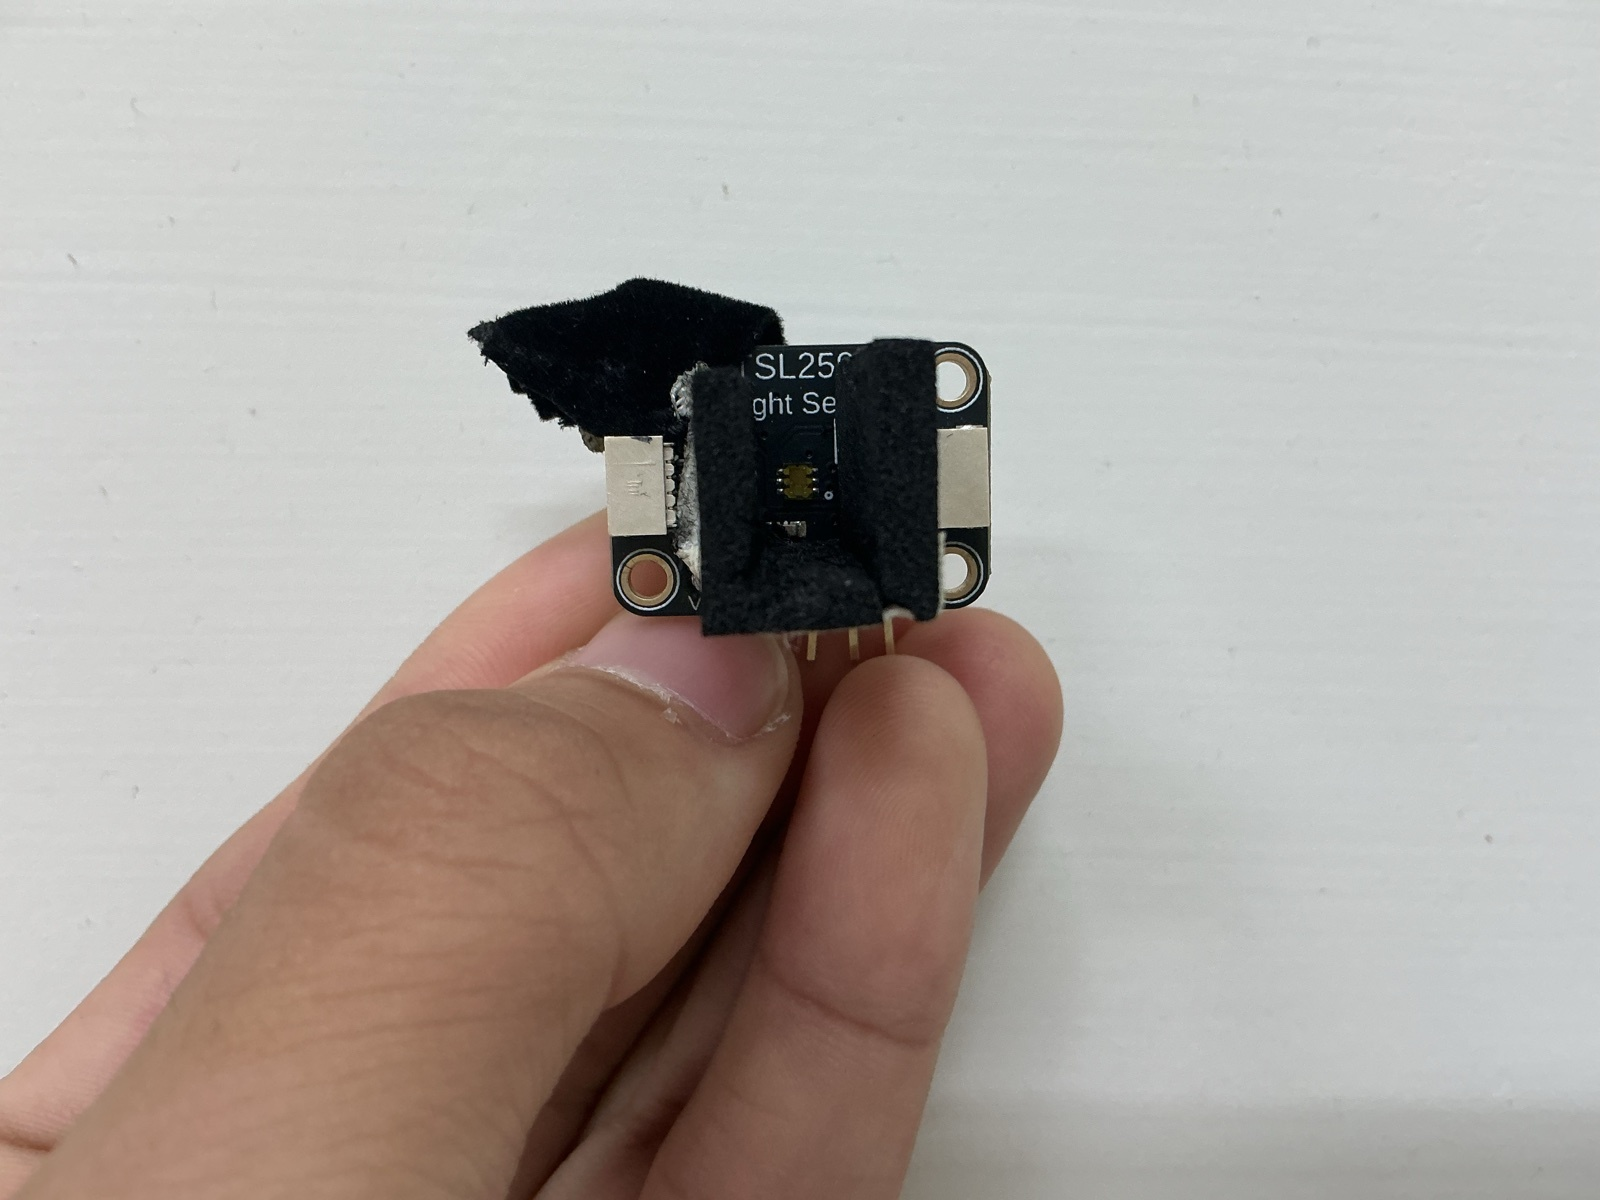
\includegraphics[width=3cm, align=c]{image/tsl2591.jpg} & 
        \centering 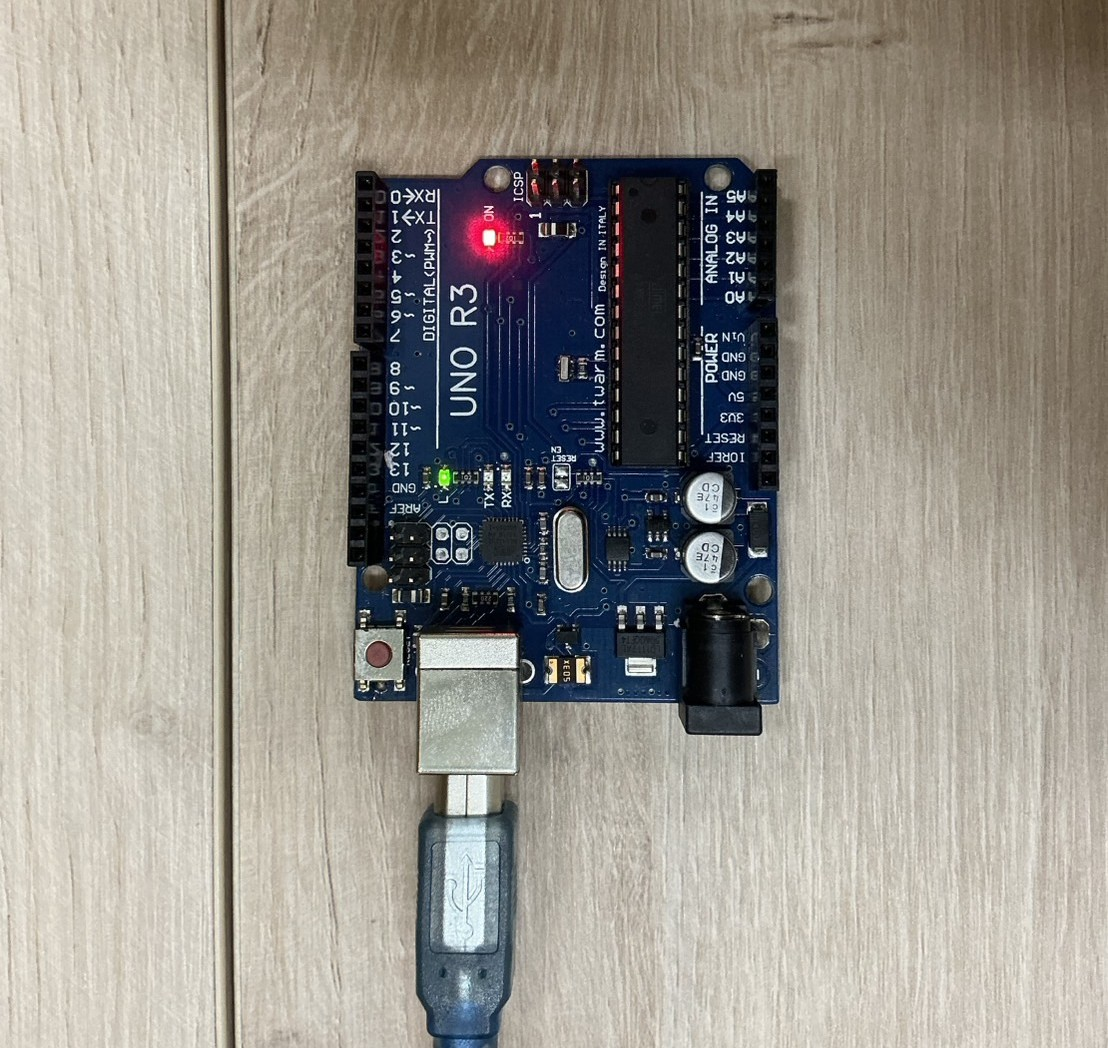
\includegraphics[width=3cm, align=c]{image/Arduino.JPG} \tabularnewline 
        \hline

        \centering 名稱 & \centering 旋轉臂 & \centering EV3 馬達模組 & 自動數據同步器  \tabularnewline 
        \hline
        \centering 圖片 & 
        \centering 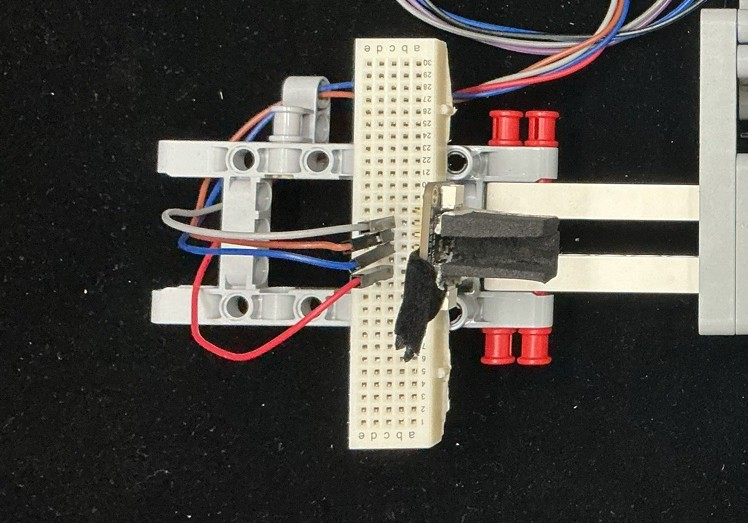
\includegraphics[width=3cm, align=c]{image/旋轉臂.jpg} & 
        \centering 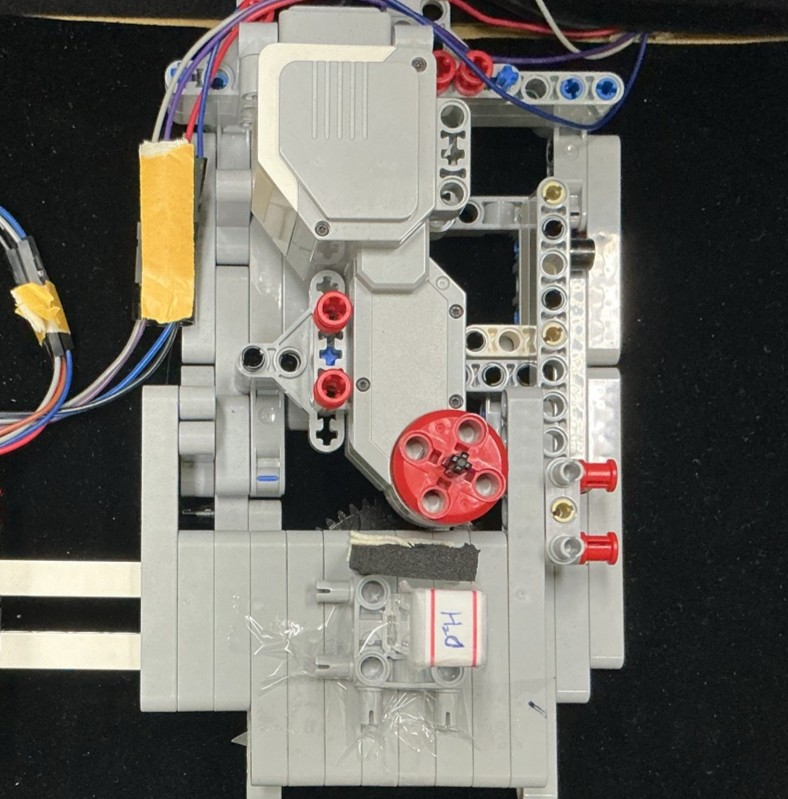
\includegraphics[width=3cm, align=c]{image/ev3.jpg} &
        \centering 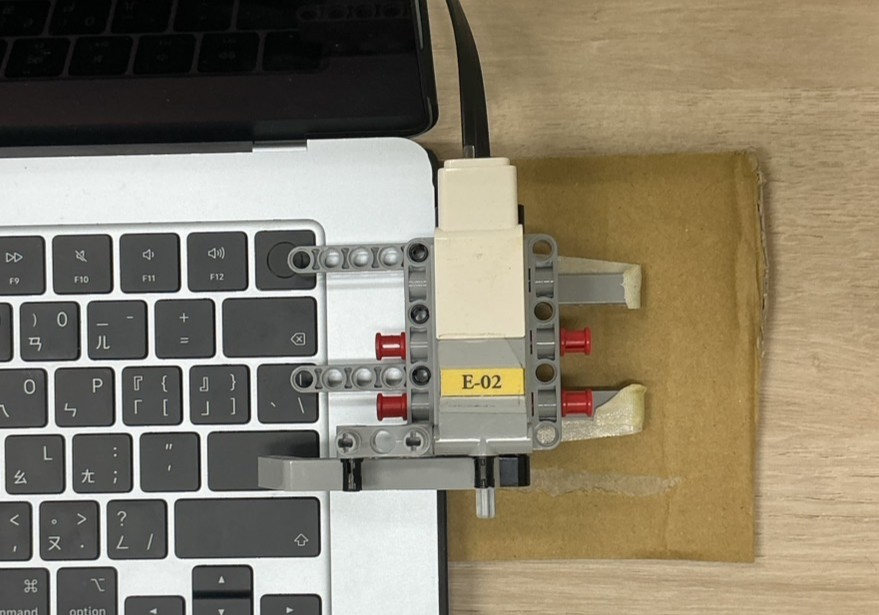
\includegraphics[width=3cm, align=c]{image/數據同步器.JPG} 
         \tabularnewline 
        \hline

        \centering 名稱 & \centering 暗室 &  &   \tabularnewline 
        \hline
        \centering 圖片 & 
        \centering 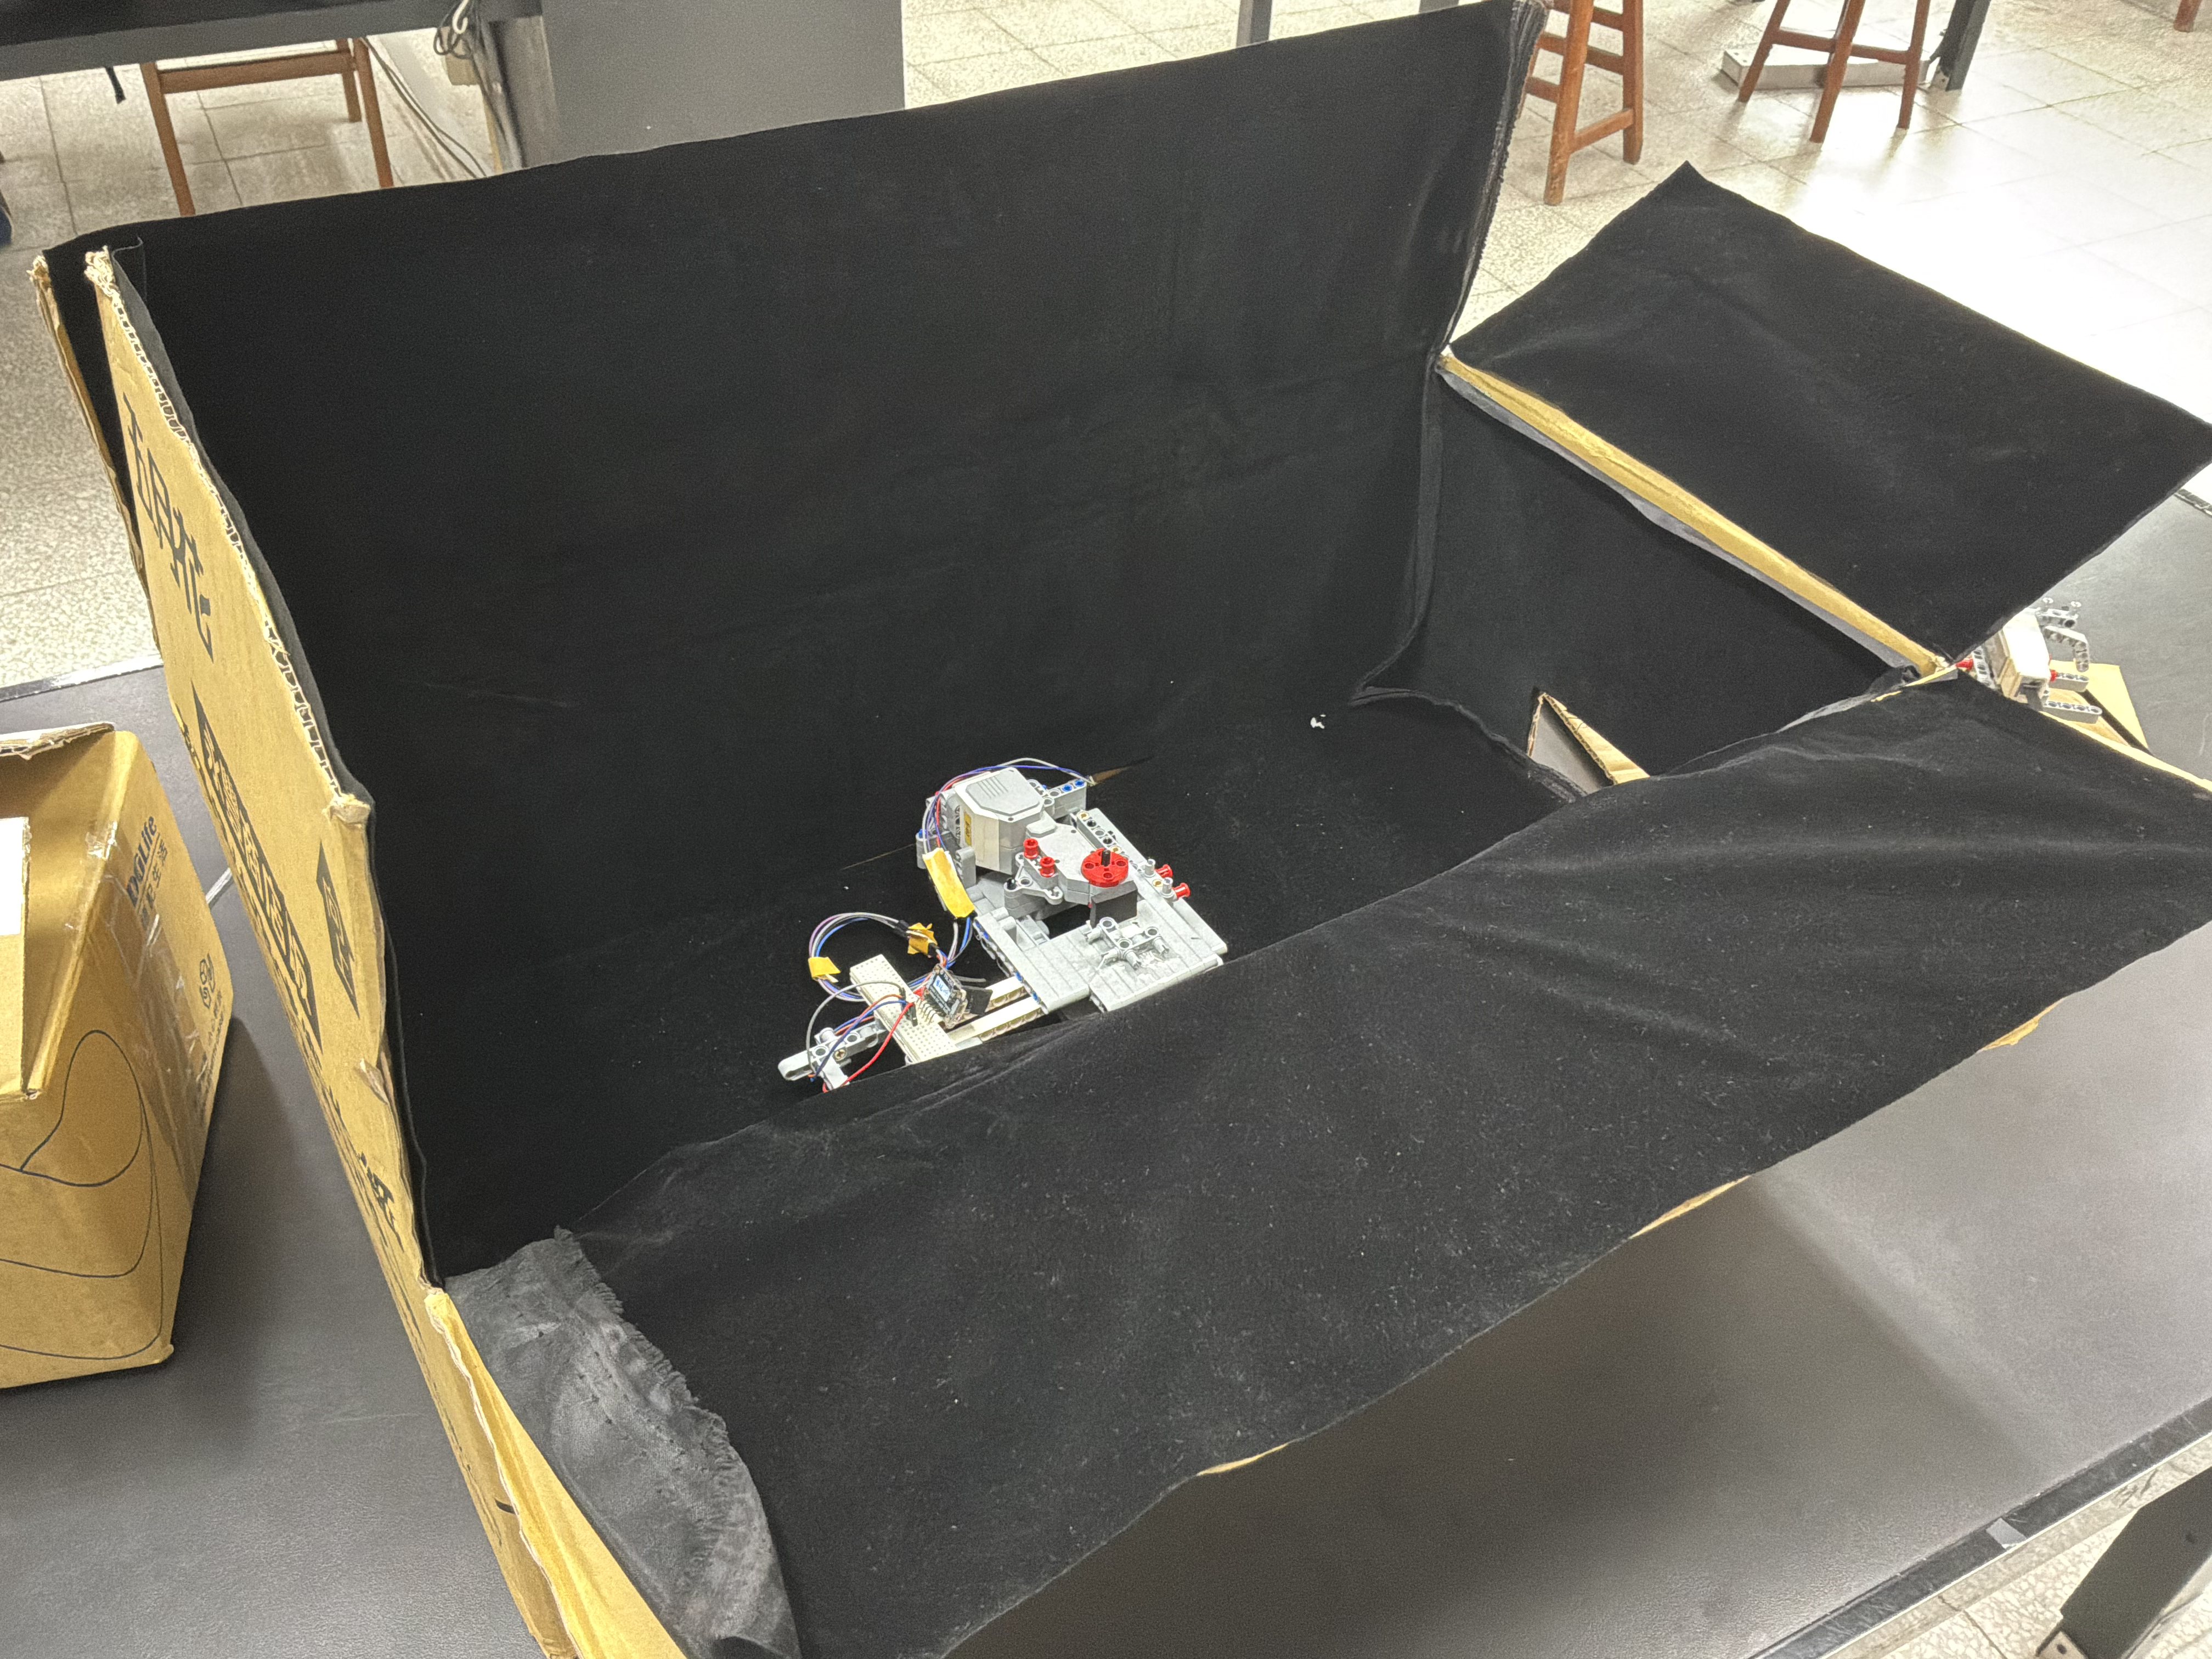
\includegraphics[width=3cm, align=c]{image/暗室.png} &  &
         \tabularnewline 
        \hline
    \end{tabular}
\end{table}
\subsubsection*{說明}
\begin{itemize}
    \item 氦氖雷射（He-Ne laser）：波長 $632.8\,\mathrm{nm}$、功率 $5\,\mathrm{mW}$，作為光源。
    \item TSL2591 數位光感測模組（Adafruit）：收光面積 $0.28\,\mathrm{mm}^2$，使用全光譜 CH0 與紅外線 CH1，並以 CH0 減 CH1 作為散射強度。
    \item Arduino Uno 微控制器：讀取感測器並將資料傳至電腦。
    \item 旋轉臂：以 LEGO Education MINDSTORMS EV3 零件組裝並由 EV3 馬達驅動，實測半徑 $110\,\mathrm{mm}$；感測器裝於臂端，每 $1^\circ$ 停留量測，臂角範圍為 $0^\circ$ 至 $140^\circ$。
    \item EV3 馬達模組：轉動旋轉臂
    \item 自動數據同步器：同步 ev3 轉動與紀錄數據的資訊
    \item 暗室 : 隔絕實驗室環境光
\end{itemize}

\subsection*{二、樣品配製器材}
\begin{table}[H]
    \setlength{\extrarowheight}{1pt}
    \centering

    \begin{tabular}{|m{2cm}|m{3cm}|m{3cm}|m{3cm}|m{3cm}|}
        \hline
        \centering 名稱 & \centering 聚苯乙烯微球 TM-P0500、TM-P1002 & 聚苯乙烯微球 TM-P0300、TM-P1003 & \centering 方形比色槽 & \centering 微量儀液劑 \tabularnewline \hline
        \centering 圖片 & 
        \centering 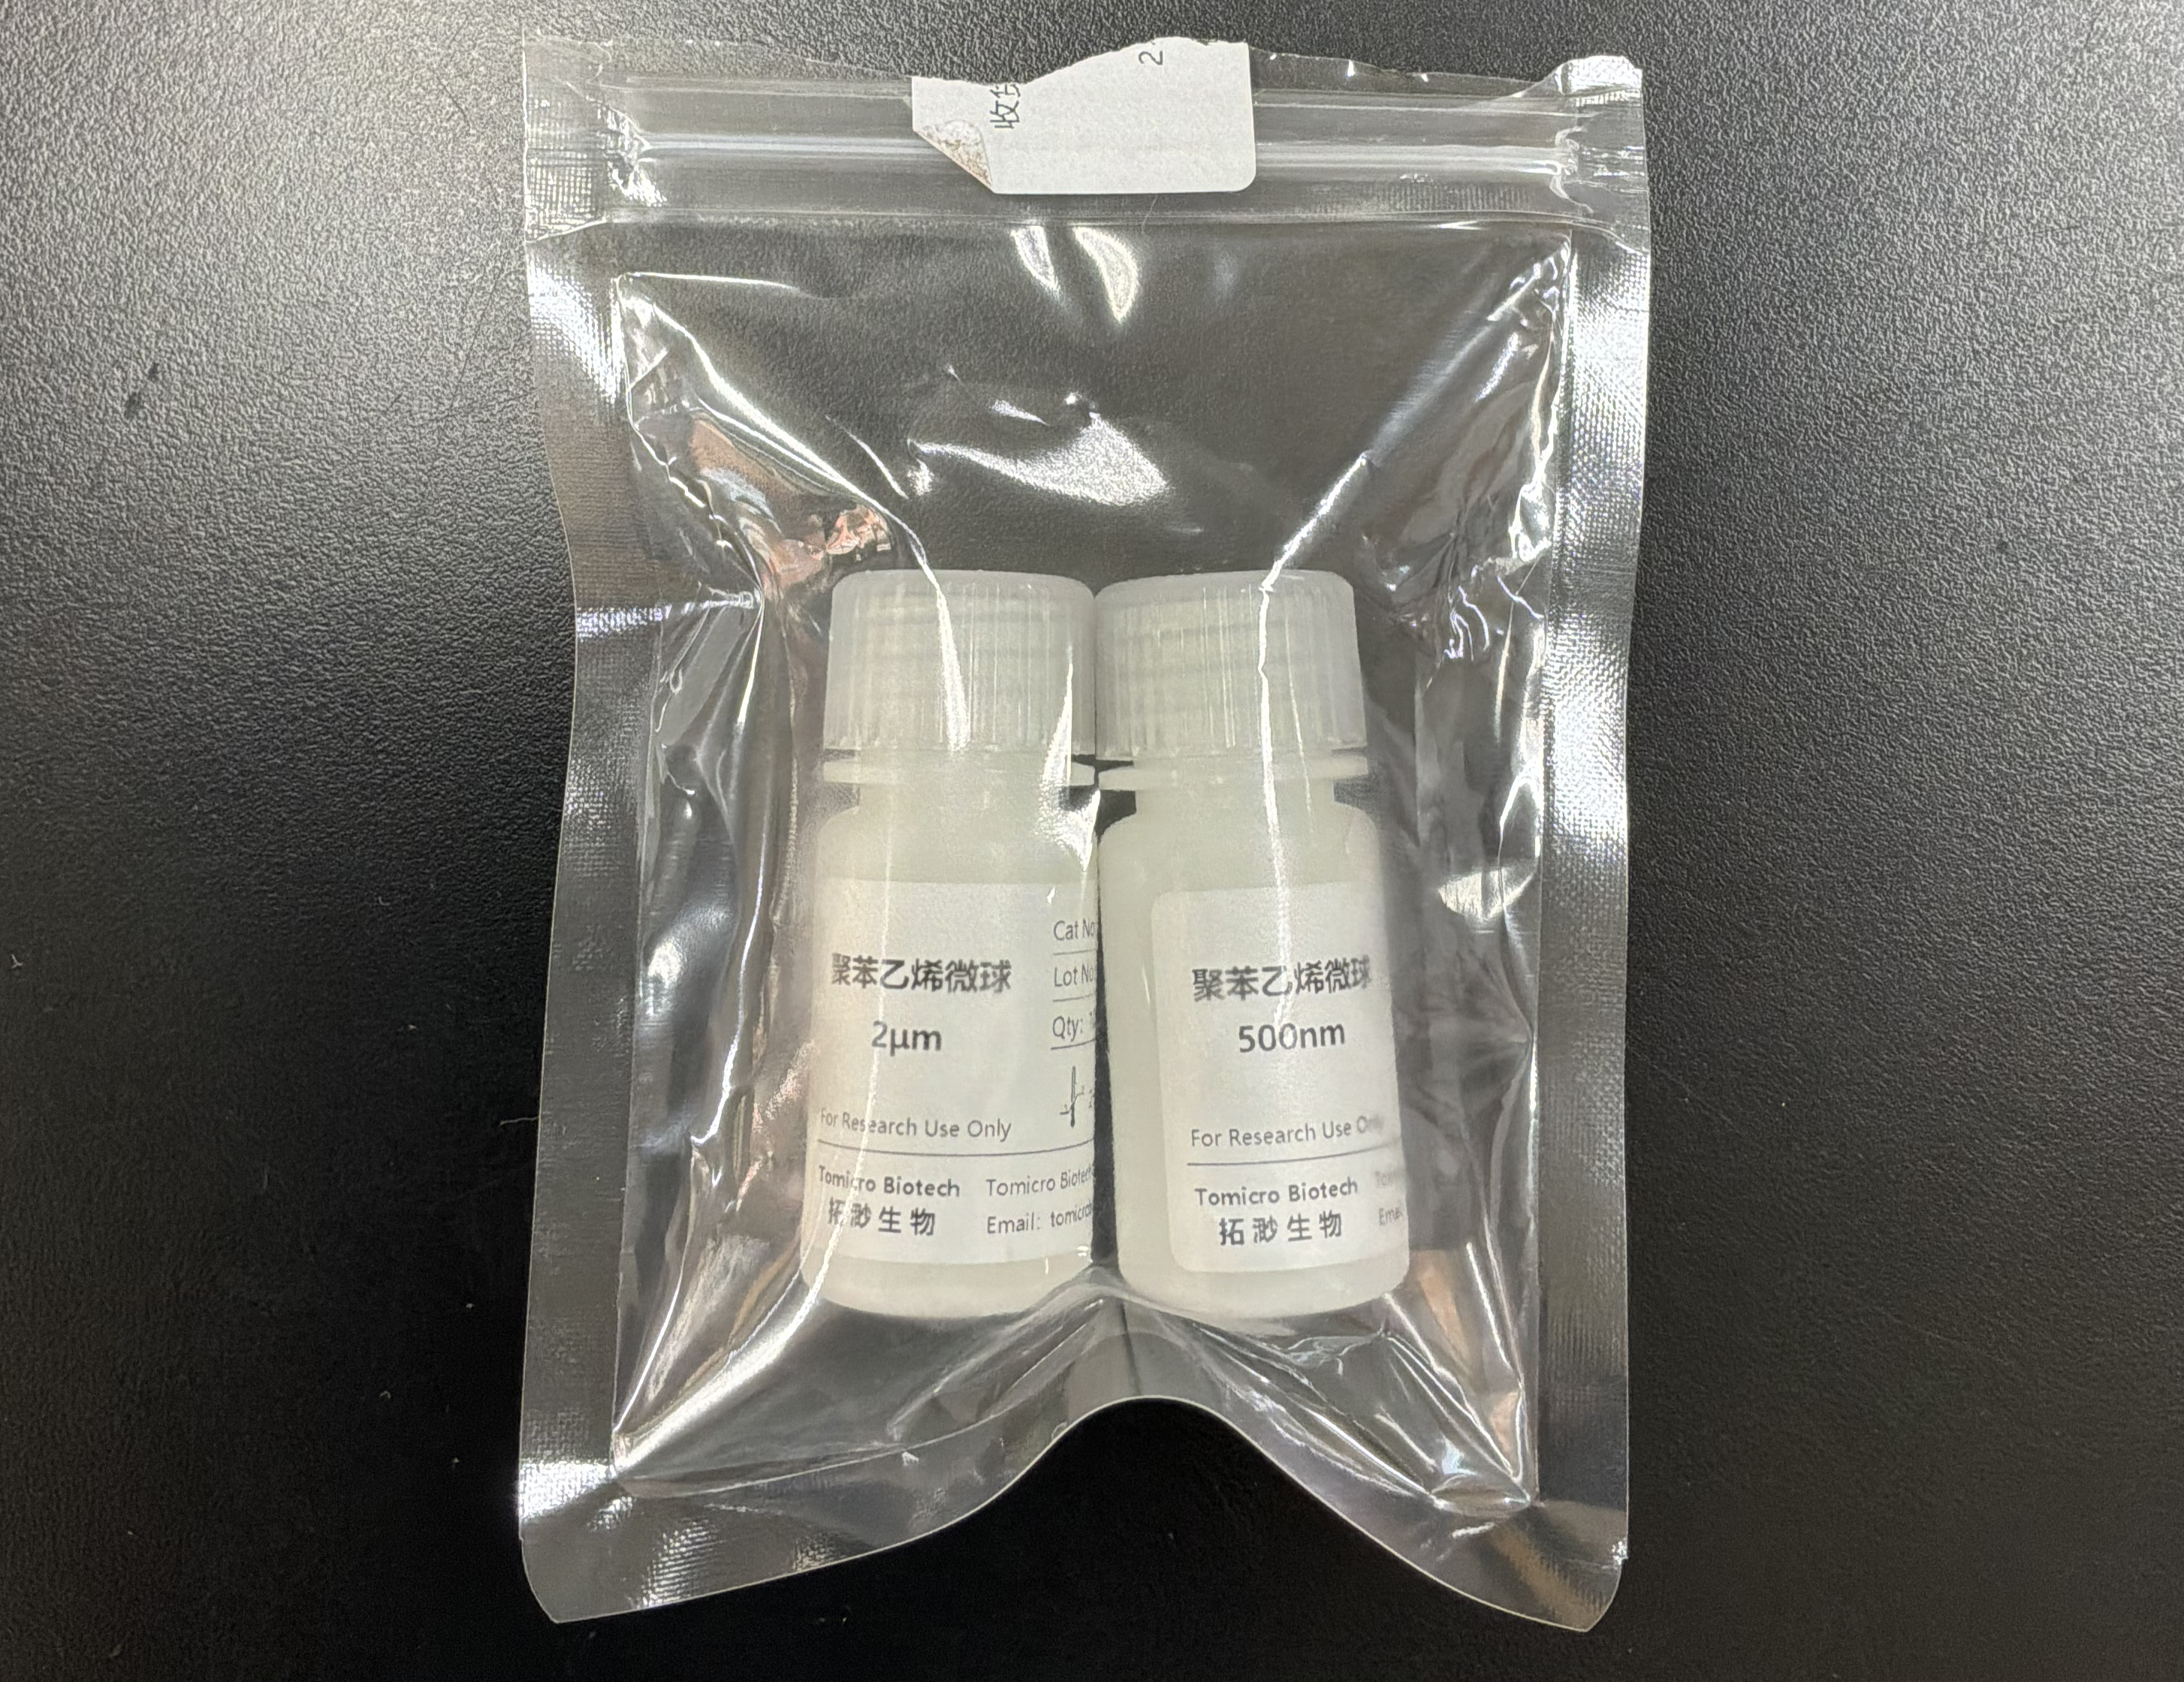
\includegraphics[width=3cm, align=c]{image/微粒 2 500.png} & 
        \centering 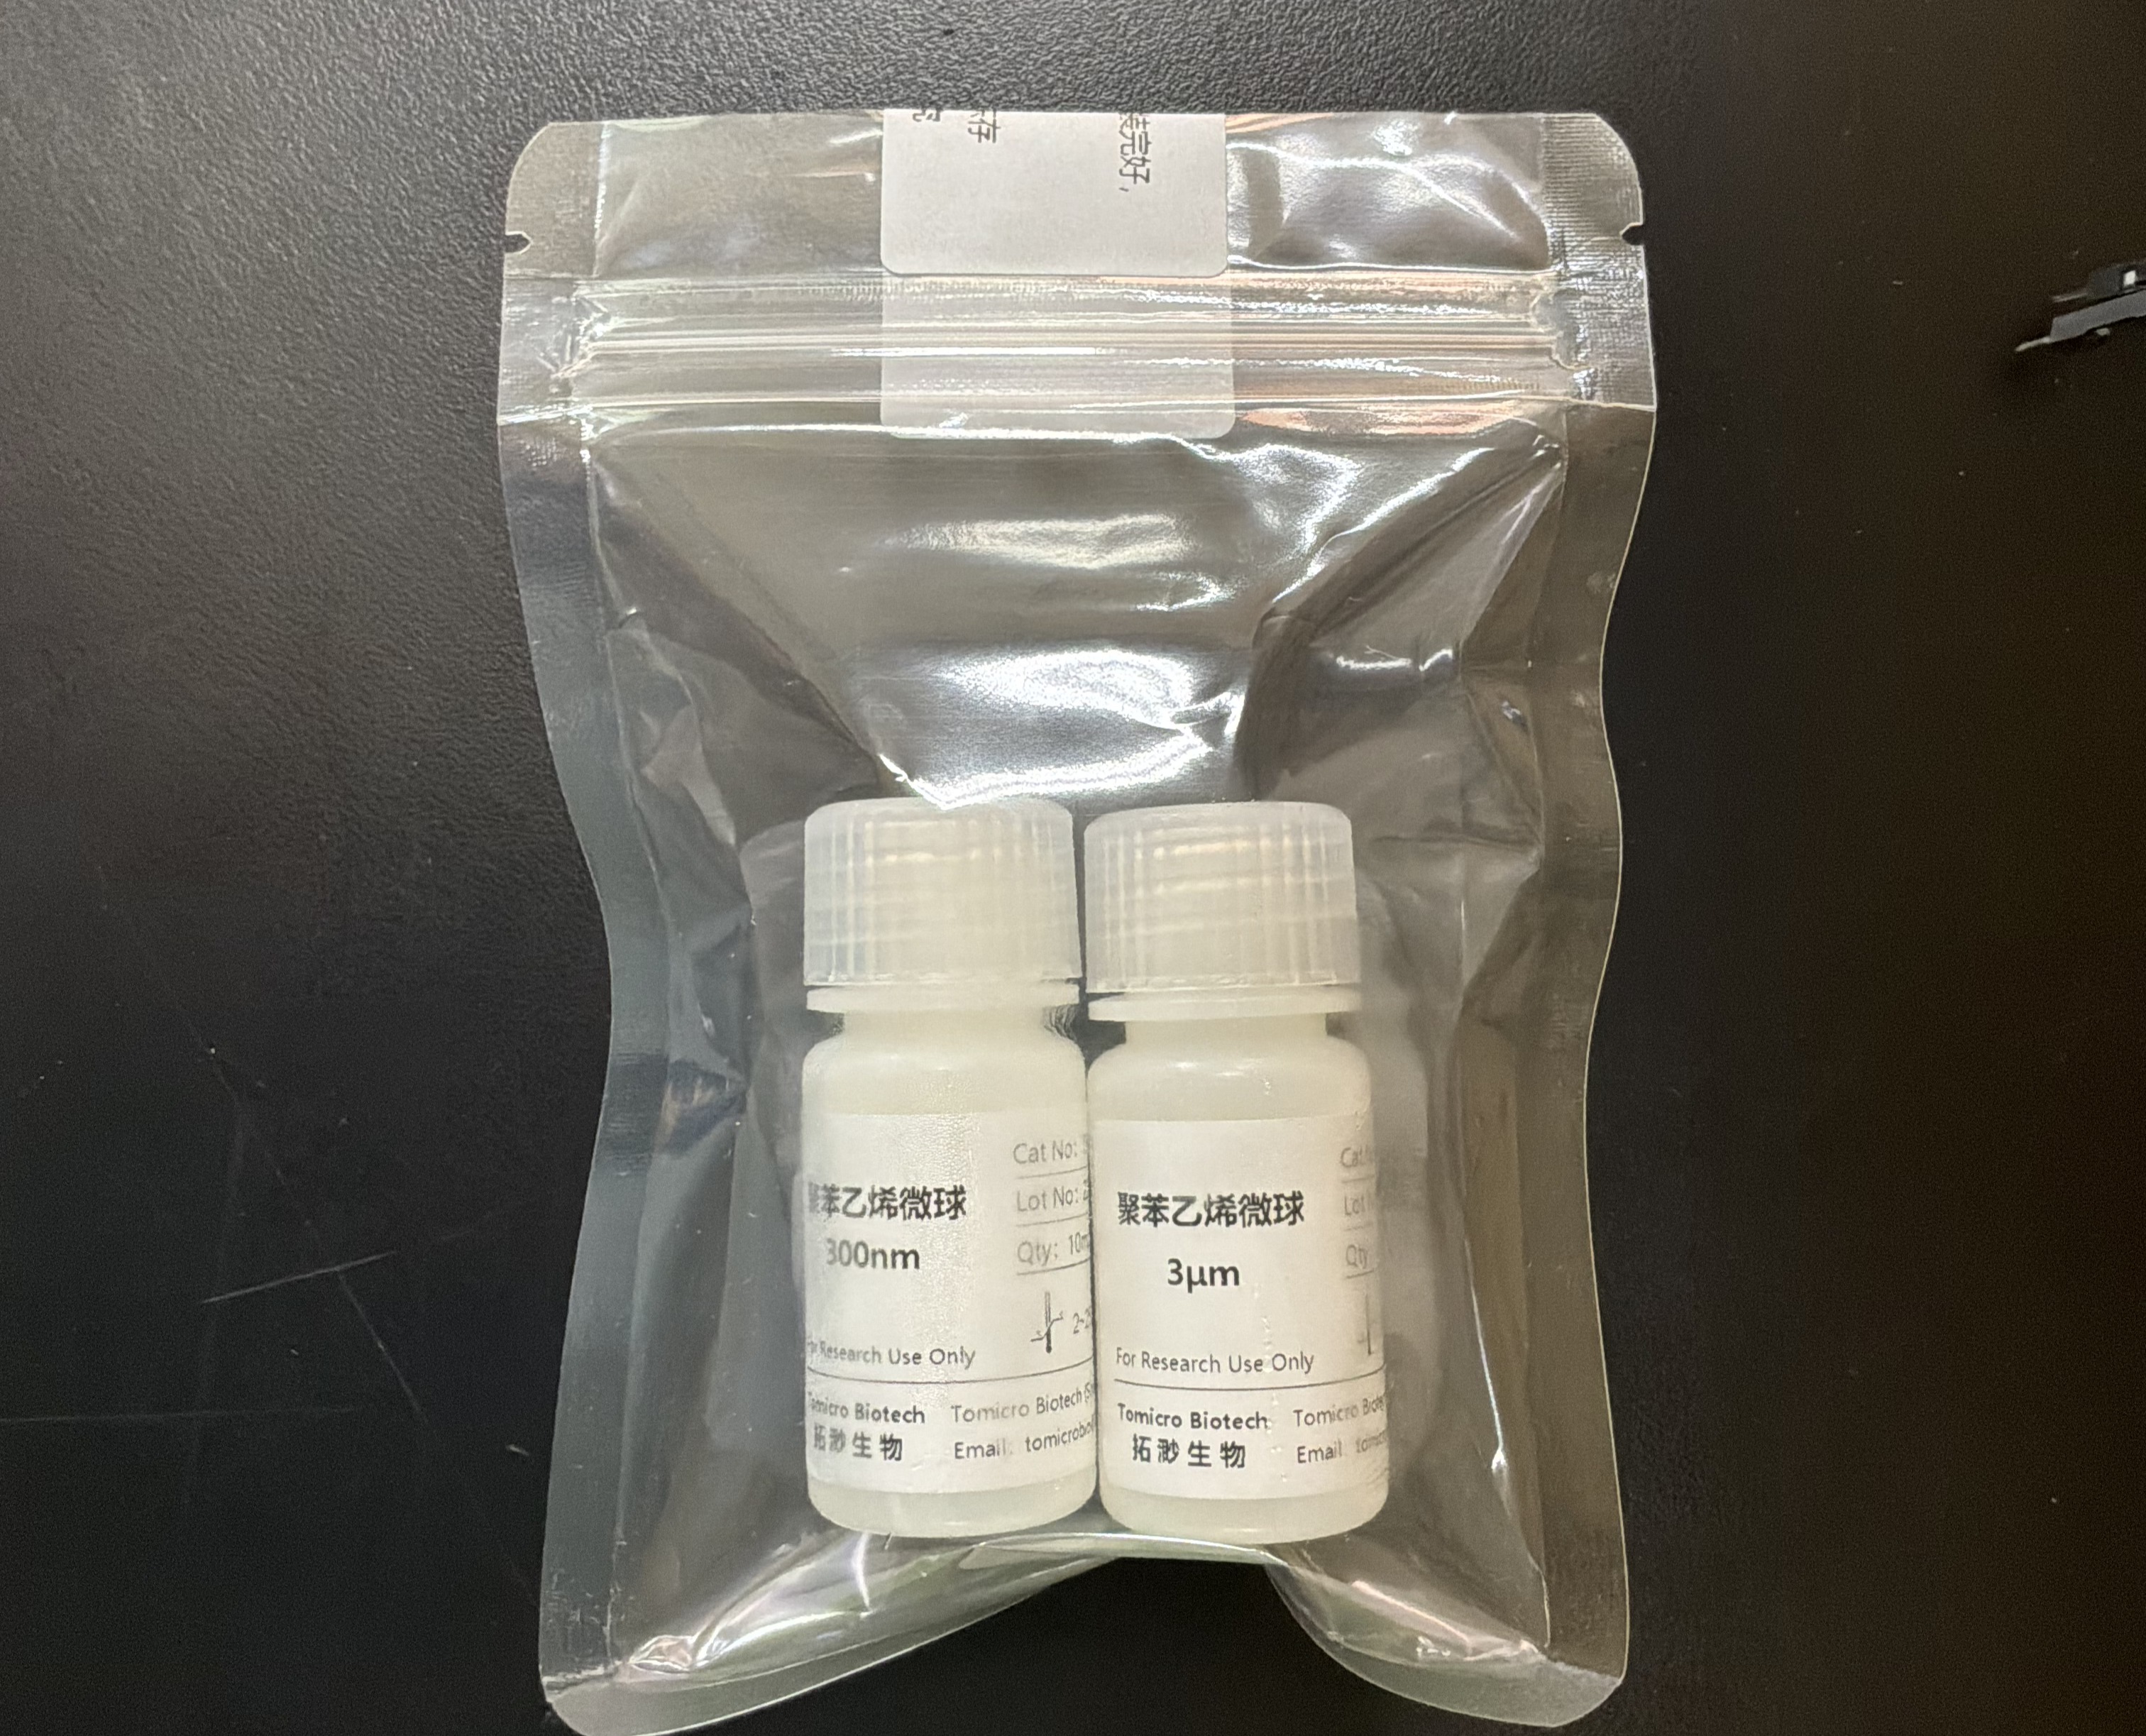
\includegraphics[width=3cm, align=c]{image/微粒 3 300.png} & 
        \centering 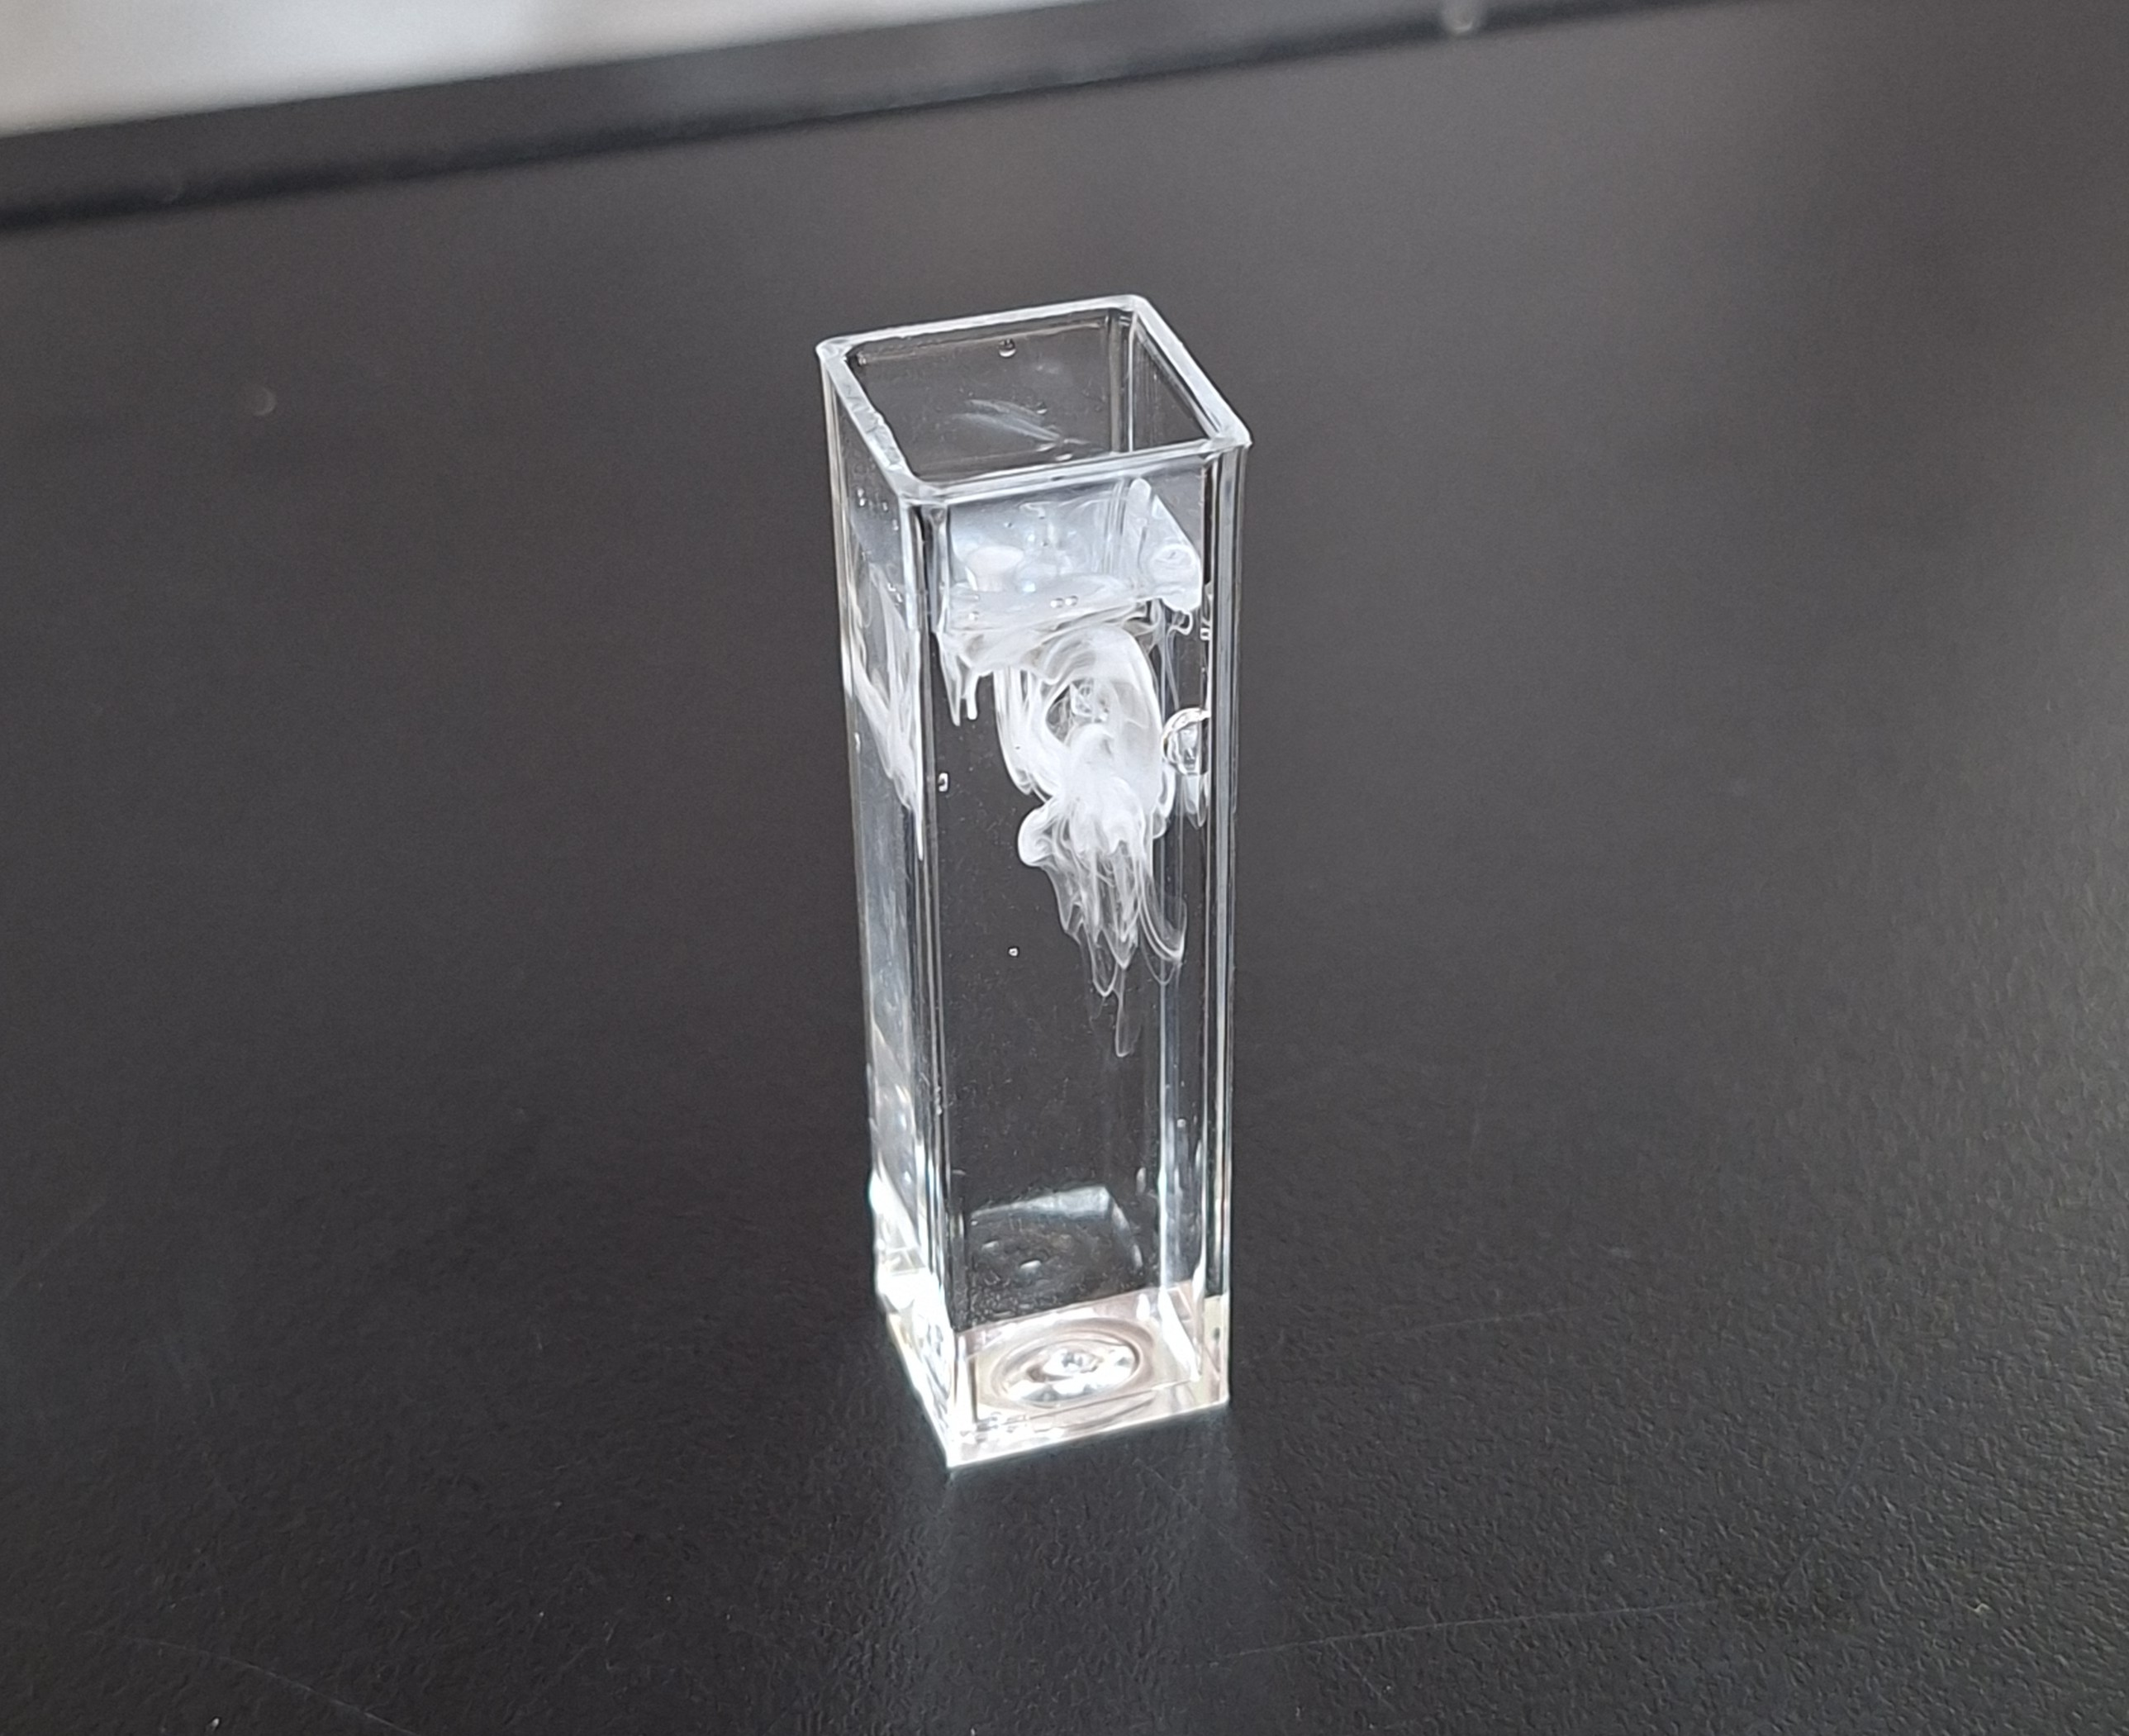
\includegraphics[width=3cm, align=c]{image/方形比色槽.jpg} &
        \centering 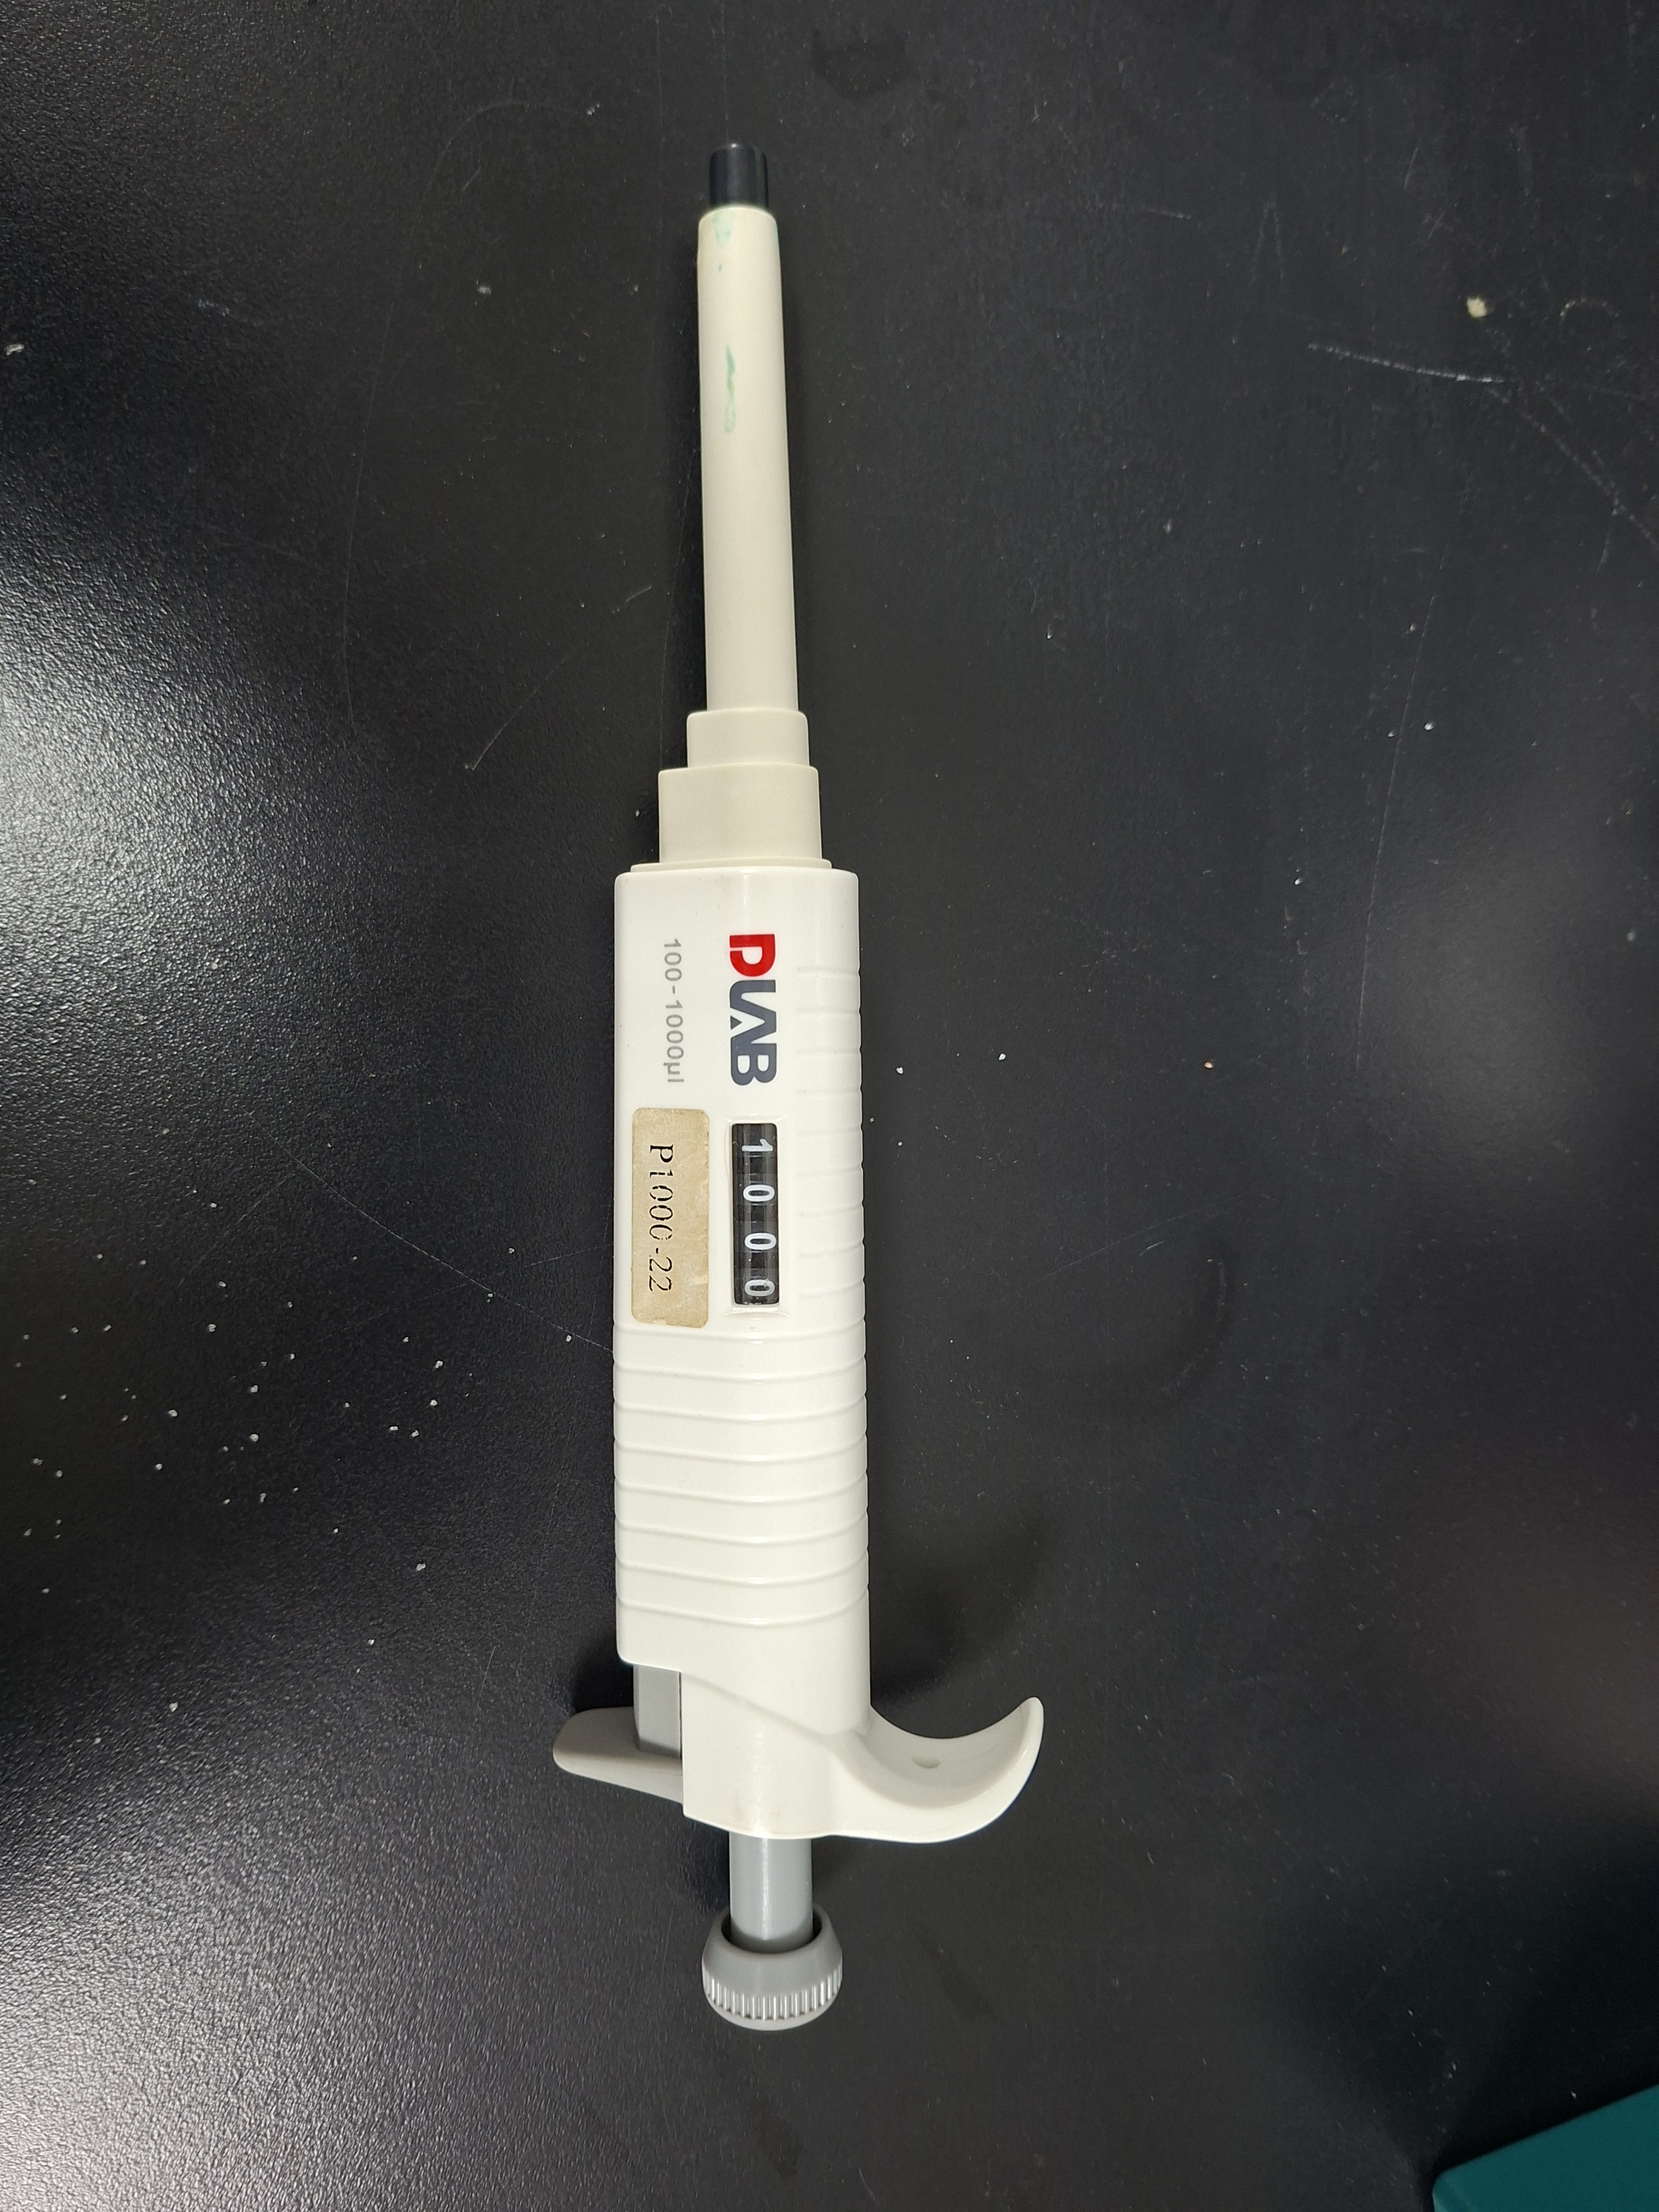
\includegraphics[width=3cm, align=c]{image/微量儀液劑 (100-1000).jpg}  \tabularnewline 
        \hline
    \end{tabular}
\end{table}

\subsubsection*{說明}
\begin{itemize}
    \item 聚苯乙烯微球 TM-P0500（拓渺 Tomicro）：實測粒徑 $492\,\mathrm{nm}$、變異係數（coefficient of variation, CV）$2.1\%$、母液質量濃度 $25\,\mathrm{mg/mL}$。
    \item 聚苯乙烯微球 TM-P1002（拓渺 Tomicro）：實測粒徑 $2.16\,\mu\mathrm{m}$、CV $3.1\%$、母液質量濃度 $25\,\mathrm{mg/mL}$。
    \item Kartell PMMA 方形比色槽：四面透光，光徑 $10\,\mathrm{mm}$，盛裝樣品。
    \item 微量吸管兩支：取母液用吸管最小刻度為 $0.1\,\mu\mathrm{L}$，取水用吸管最小刻度為 $1\,\mu\mathrm{L}$。
    \item 去離子水：作為稀釋用水及空白樣品。
\end{itemize}

\subsection*{三、雷射線偏振角度測量}
\begin{table}[H]
    \setlength{\extrarowheight}{1pt}
    \centering

    \begin{tabular}{|m{2cm}|m{3cm}|m{3cm}|m{3cm}|}
        \hline
        \centering 名稱 & \centering 無偏振雷射筆 & \centering 偏振片 & \centering 支撐架 \tabularnewline \hline
        \centering 圖片 & 
        \centering 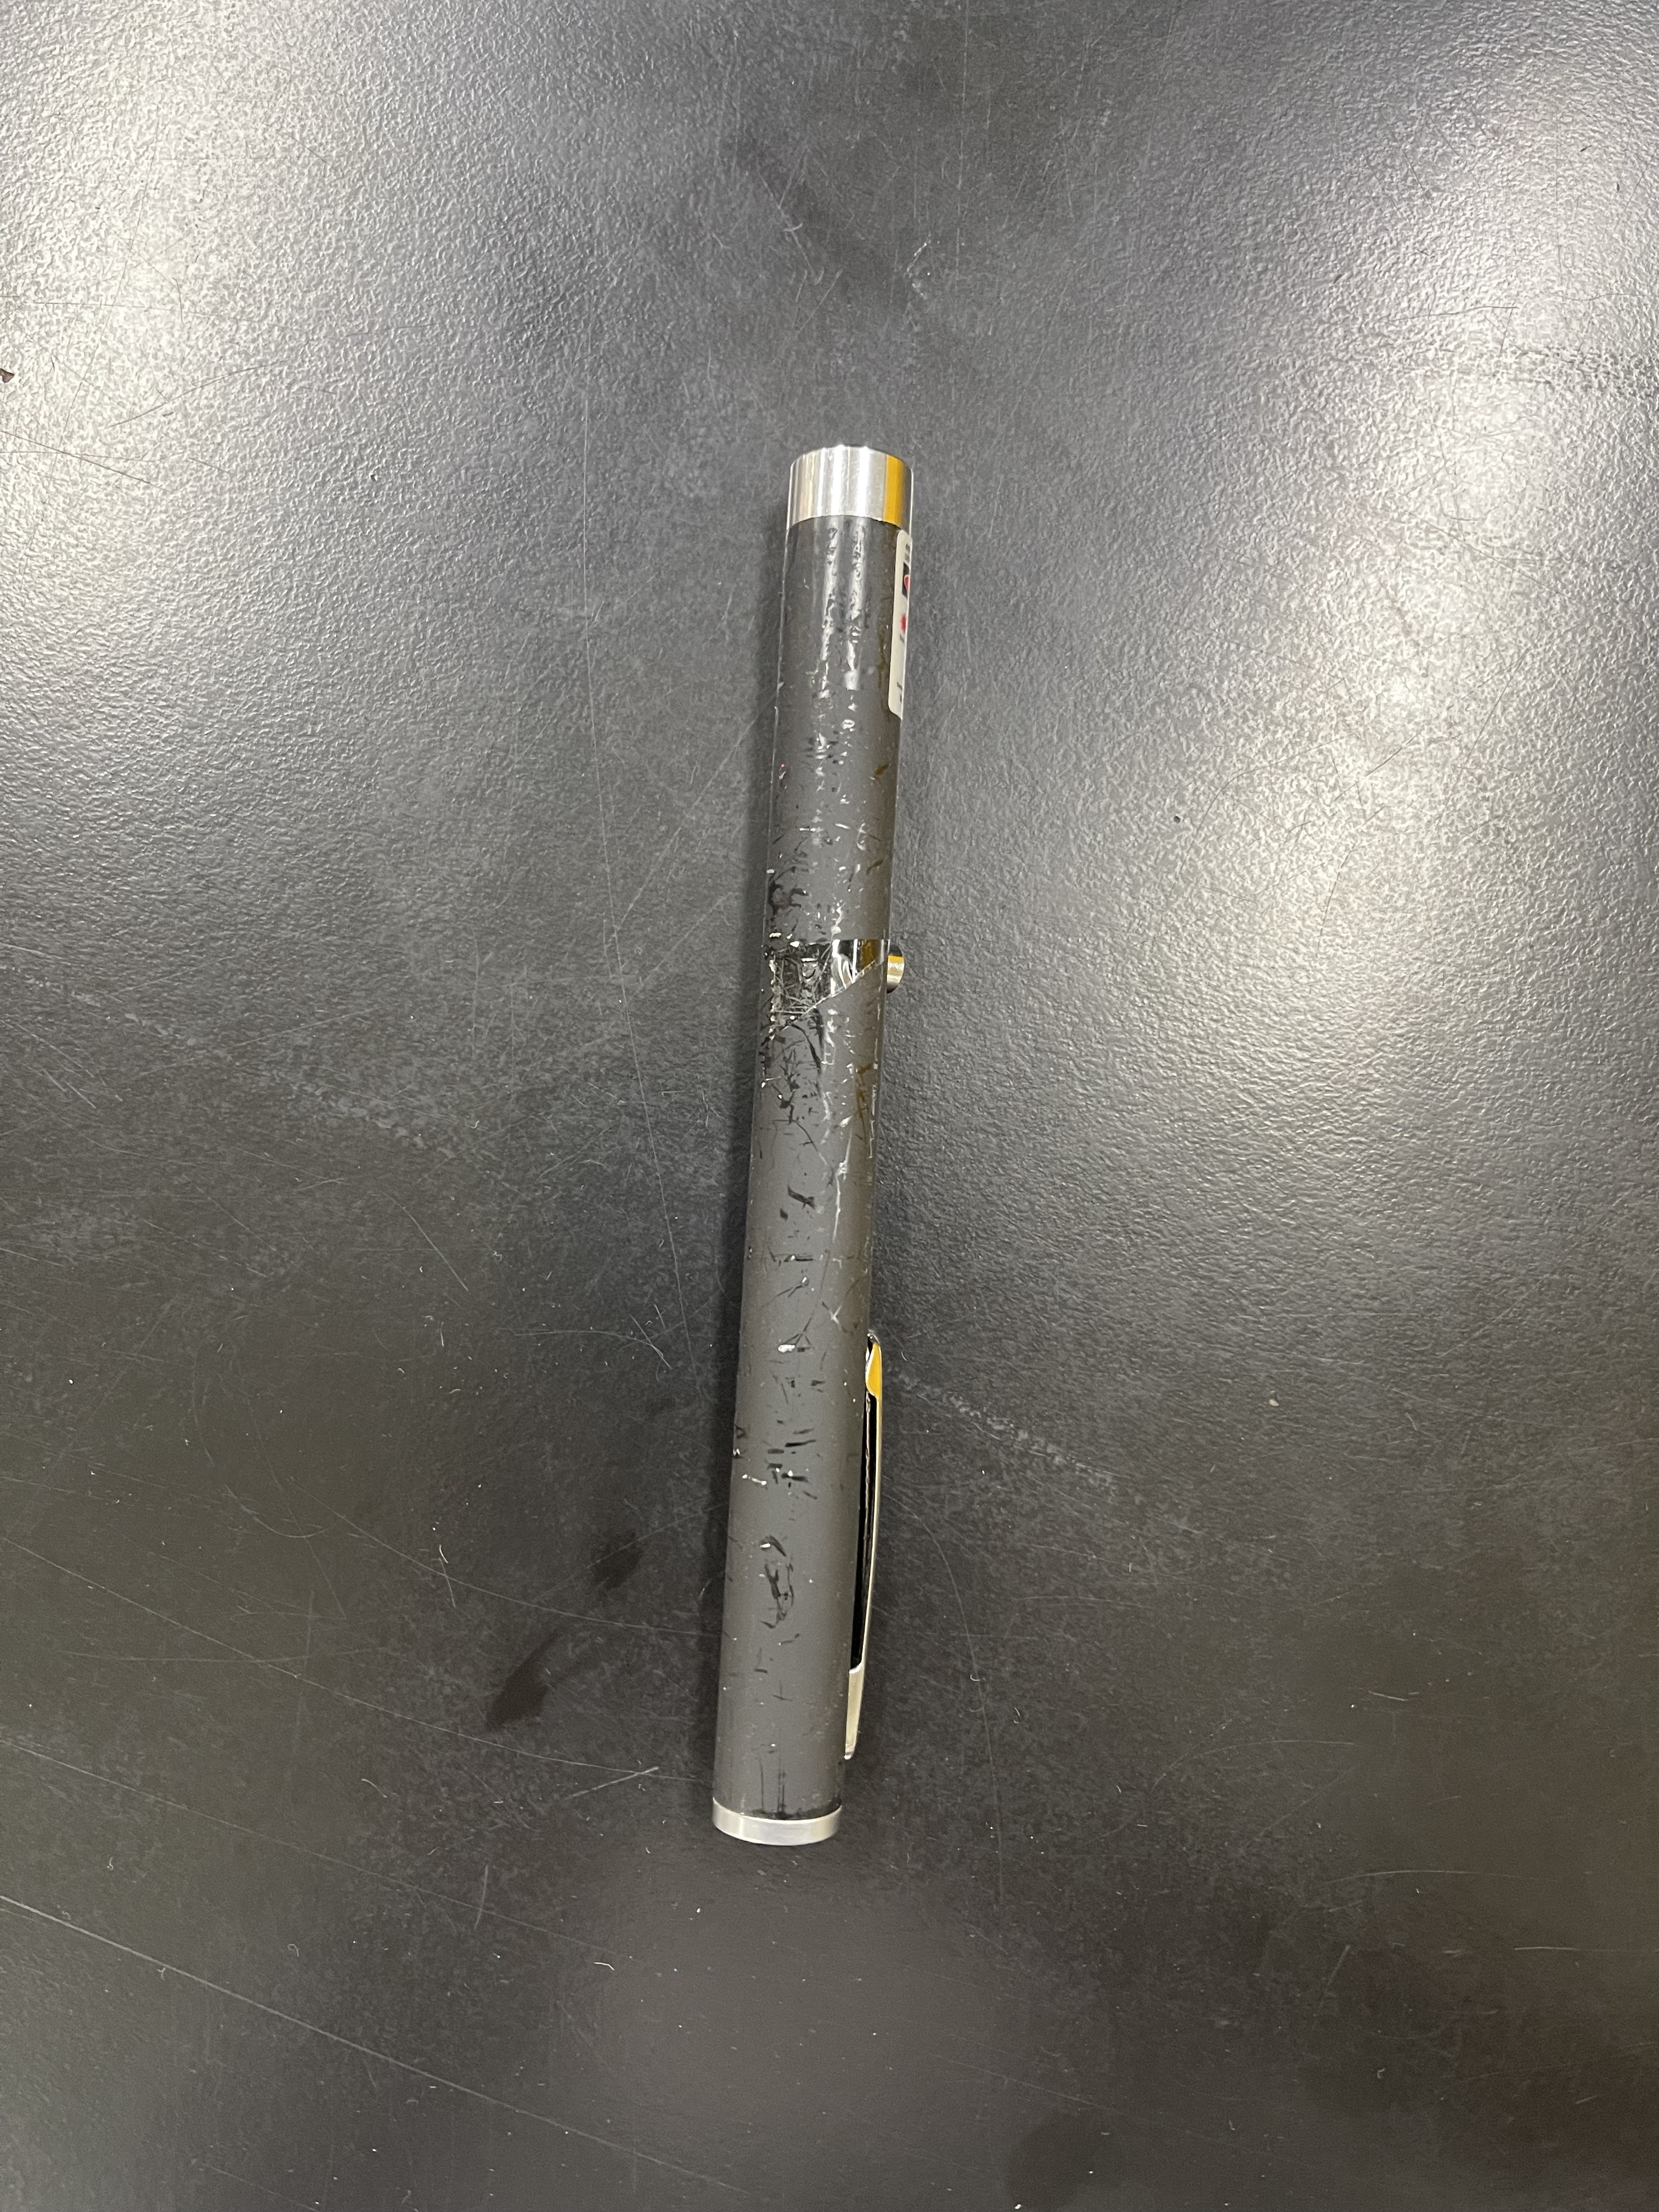
\includegraphics[width=3cm, align=c]{image/雷射筆.jpg} & 
        \centering 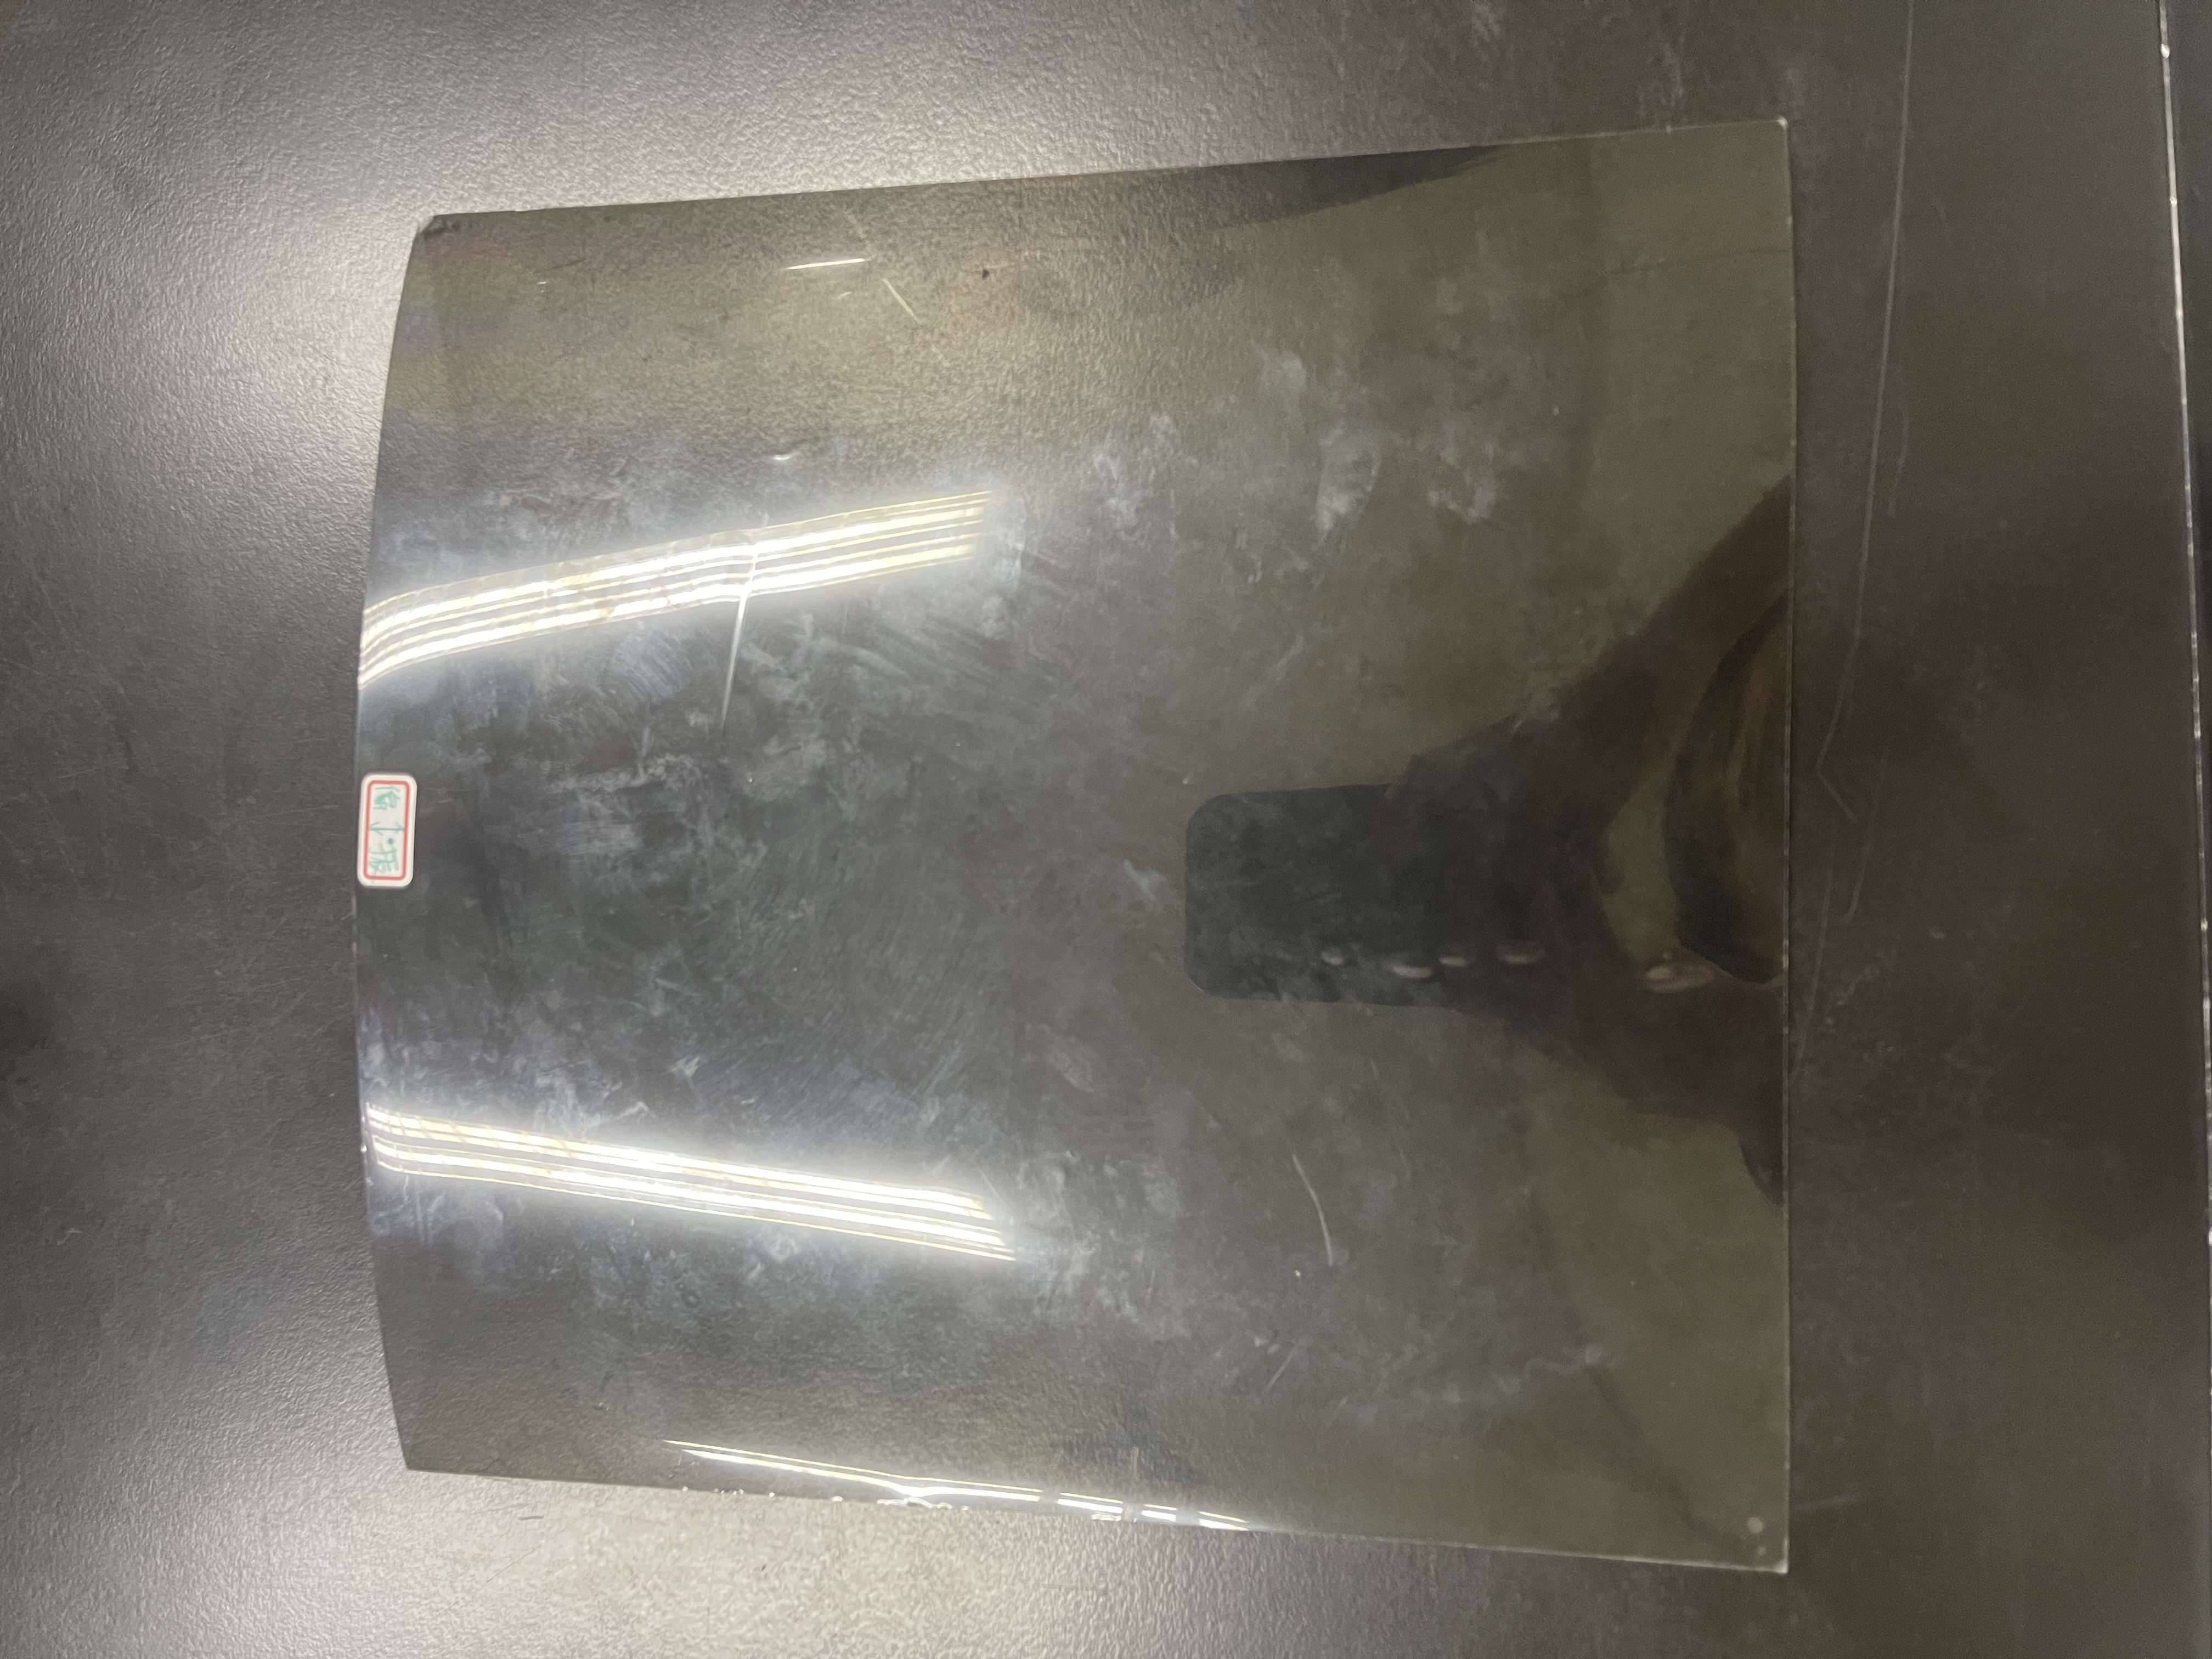
\includegraphics[width=3cm, align=c]{image/偏振片.jpg} & 
        \centering 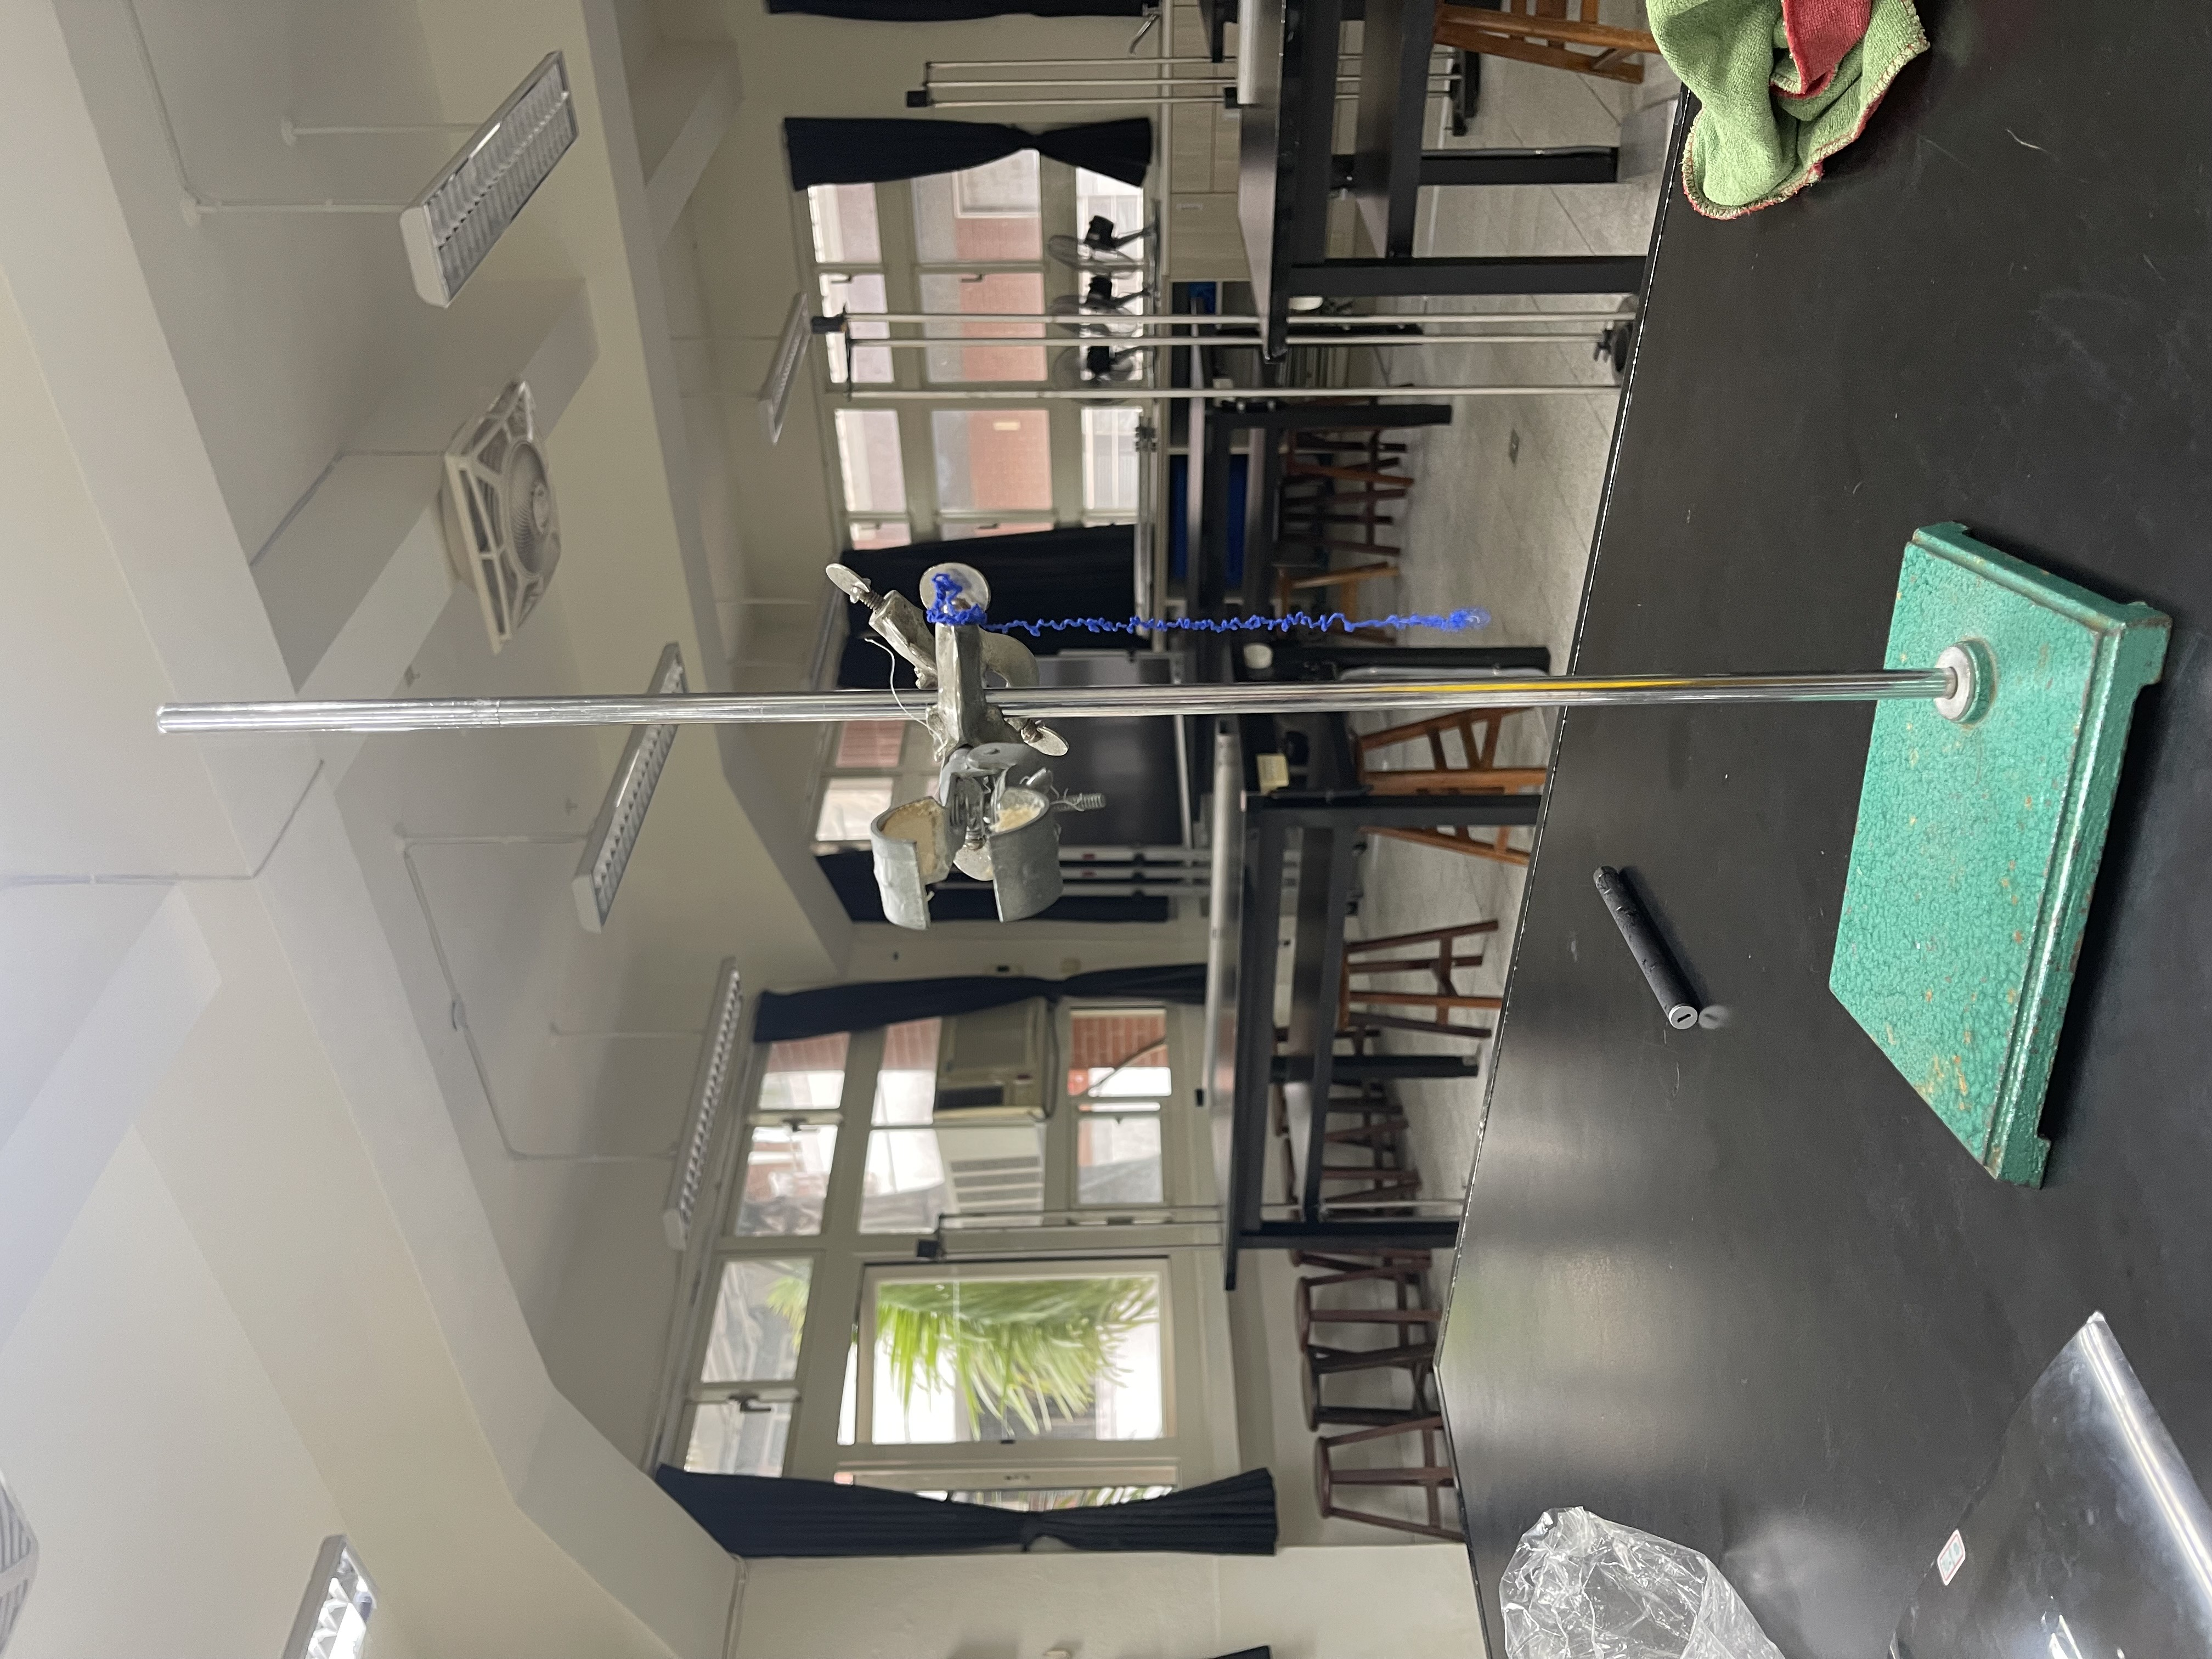
\includegraphics[width=3cm, align=c]{image/角度測量 架子.jpg} \tabularnewline 
        \hline

    \end{tabular}
\end{table}

\subsubsection*{說明}
\begin{enumerate}
    \item 無偏振雷射筆: 任意角度皆有偏振的雷射筆，用於提供入射光
    \item 偏振片: 線偏振偏振片
    \item 支撐架: 固定雷射筆使其入射角維持在布魯斯特角
\end{enumerate}


\subsection*{四、軟體使用}
\begin{table}[H]
    \setlength{\extrarowheight}{1pt}
    \centering
    
    \begin{tabular}{|m{2cm}|m{3cm}|m{3cm}|m{3cm}|}
        \hline
        \centering 名稱 & \centering Python 3.12 & \centering miepython & \centering 自製蒙地卡羅程式 \tabularnewline \hline
        \centering 圖片 & 
        \centering 
\includegraphics[width=2.3cm, align=c]{image/python.jpg} & 
        \centering 
\includegraphics[width=3cm, align=c]{image/miepython.png} & 
        \centering 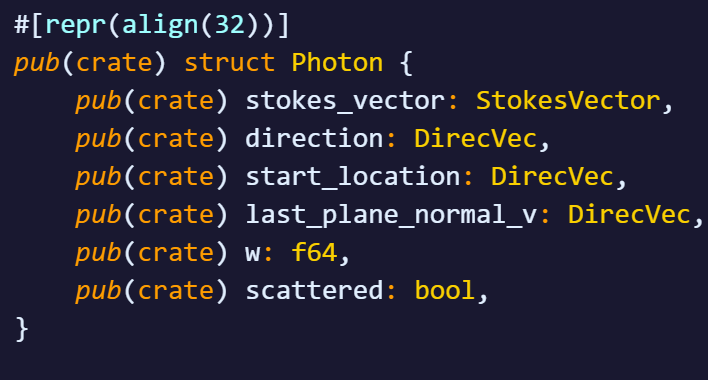
\includegraphics[width=3cm, align=c]{image/蒙地卡羅.png} \tabularnewline 
        \hline

        \centering 名稱 & \centering LEGO EV3 & \centering  rustc 1.98.0 &  \tabularnewline \hline
        \centering 圖片 & 
        \centering 
\includegraphics[width=2.5cm, align=c]{image/ex3_logo.jpg} & 
        \centering 
\includegraphics[width=2.5cm, align=c]{image/rust.png} & \tabularnewline 
        \hline
    \end{tabular}
\end{table}
\subsubsection*{說明}
\begin{itemize}
    \item Python 3：數據處理，包括角度切割、空白扣除、計算 $C$ 與不確定度。
    \item miepython：計算 Mie 散射效率 $Q_{\mathrm{sca}}$、異向性參數 $g$ 與相位函數。
    \item 自製蒙地卡羅程式：模擬多重散射。
    \item LEGO MINDSTORMS EV3 官方軟體：控制旋轉臂每 $1^\circ$ 停留量測。
    \item Rust：撰寫序列埠監測程式並儲存感測資料。
\end{itemize}